%% Adaptado a partir de :
%%    abtex2-modelo-trabalho-academico.tex, v-1.9.2 laurocesar
%% para ser um modelo para os trabalhos no IFSP-SPO

\documentclass[
    % -- opções da classe memoir --
    12pt,               % tamanho da fonte
    openright,          % capítulos começam em pág ímpar (insere página vazia caso preciso)
    %twoside,            % para impressão em verso e anverso. Oposto a oneside
    oneside,
    a4paper,            % tamanho do papel. 
    % -- opções da classe abntex2 --schwinn
    % Opções que não devem ser utilizadas na versão final do documento
    %draft,              % para compilar mais rápido, remover na versão final
    paginasA3,  % indica que vai utilizar paginas em A3 
    BIBLATEX,           % indica para utilizar BIBLATEX em vez do abntex2cite
    REFINDENT,          % não fica exatamente no formato da ABNT, mas melhora muito a formatação
                        % não utilizar REFINDENT na versão final
    MODELO,             % indica que é um documento modelo então precisa dos geradores de texto
    %TODO,               % indica que deve apresentar lista de pendencias 
    % -- opções do pacote babel --
    english,            % idioma adicional para hifenização
    brazil              % o último idioma é o principal do documento
    ]{ifsp-spo-inf-cemi} % ajustar de acordo com o modelo desejado para o curso
%\AtBeginDocument{\todo[inline]{Ajustar a classe de referencia de documentclass no inicio do arquivo principal de acordo com o curso do(s) aluno(s)}}

% ---
% Informações de dados para CAPA e FOLHA DE ROSTO
% ---
\titulo{Metaverso - Ferramenta de Chamados de TI (ITSM) para pessoas físicas e pequenas empresas}

% Trabalho individual
%\autor{AUTOR DO TRABALHO}

% Trabalho em Equipe
% ver também https://github.com/abntex/abntex2/wiki/FAQ#como-adicionar-mais-de-um-autor-ao-meu-projeto
\renewcommand{\imprimirautor}{
	\begin{tabular}{lr}
		%CEZAR GODOY NASCIMENTO	& SP3040755 \\
		HENRIQUE HIROMI SHIMADA & SP3039421 \\
		ISABELA SOUZA DUARTE	& SP3030083 \\
		MATEUS SOUZA DA SILVA	& SP3022374 \\
		VINICIUS GOMES MOREIRA	& SP3039587 \\
		WELEN MOTA SOUSA		& SP146616X \\
	\end{tabular}
}


\disciplina{PI1A5 - Projeto Integrado I}

\data{ABRIL DE 2022}

% Definir o que for necessário e comentar o que não for necessário
% Utilizar o Nome Completo, abntex tem orientador e coorientador
% então vão ser utilizados na definição de professor
\renewcommand{\orientadorname}{Professor:}
\orientador{JOSE BRAZ DE ARAUJO}
\renewcommand{\coorientadorname}{Professor:}
\coorientador{MARCELO TAVARES DE SANTANA}


% ---


% informações do PDF
\makeatletter
\hypersetup{
        %pagebackref=true,
        pdftitle={\@title}, 
        pdfauthor={\@author},
        pdfsubject={\imprimirpreambulo},
        pdfcreator={LaTeX with abnTeX2 using IFSP model},
        pdfkeywords={abnt}{latex}{abntex}{abntex2}{IFSP}{\ifspprefixo}{trabalho acadêmico}, 
        colorlinks=true,            % false: boxed links; true: colored links
        linkcolor=blue,             % color of internal links
        citecolor=blue,             % color of links to bibliography
        filecolor=magenta,              % color of file links
        urlcolor=blue,
        bookmarksdepth=4
}
\makeatother
% --- 

% carregando aqui referencias quando utilizando BIBLATEX
\IfPackageLoaded{biblatex}{%
\addbibresource{referencias.bib}
\addbibresource{exemplos/abntex2-doc-abnt-6023.bib}
}{}

% ----
% Início do documento
% ----
\begin{document}



% Retira espaço extra obsoleto entre as frases.
\frenchspacing 

%somente para o exemplo, fica primeiro
\todo[inline]{Remover texto informativo inicial}
%

Esse documento foi feito a partir do modelo canônico de trabalho acadêmico da classe \abnTeX, o acesso projeto com fontes e ao \acs{pdf} pode ser feito em 
\urlmodelo. Esse modelo foi feito como exemplo para alunos dos cursos de informática do \ac{ifsp}. Um modelo para apresentações (\textit{slides}) utilizando Beamer está disponível em  \url{https://www.overleaf.com/read/qjrjhqwqbqqw}


Este documento não pode ser considerado como um padrão a ser seguido em sua totalidade, ele tem como maior objetivo demonstrar como utilizar o \LaTeX\ para obter um documento atendendo ao máximo o padrão do \ac{ifsp} e \ac{abnt}. Ele não foi montado como um curso de {\LaTeX} já que existem diversos disponíveis na internet. O formato textual está mais próximo de um manual do que a um trabalho acadêmico.

Esse modelo é atualizado constantemente tentando apresentar e resolver problemas que aparecem nos trabalhos das disciplinas. Se você encontrar um problema ou inconsistência envie a informação para o seu professor de informática do \ac{ifsp}. Portanto é importante sempre utilizar a ultima versão dos arquivos de classe (\textbf{.cls}) deste modelo em seu documento de forma a utilizar todos os ajustes e configurações aplicados nesse documento.

O formato geral de cada trabalho a ser desenvolvido depende do contexto, mas os principais capítulos de todos os trabalhos são : Introdução, Revisão de Literatura, em seguida os capítulos referentes ao desenvolvimento do trabalho e finalmente as Considerações Finais.

Para entender corretamente como desenvolver seu documento em {\LaTeX} é importante fazer uma leitura dos arquivos fonte {\LaTeX} e não somente do documento \acs{pdf} gerado pelo compilador {\LaTeX}. E fazer também leitura das definições de referências (arquivos \textbf{.bib}).

Algumas bibliotecas \LaTeX\ disponíveis no overleaf estão desatualizadas, para melhores resultados é recomendável a utilização de outro compilador utilizando as ultimas versões de todas bibliotecas

Esse documento possui elementos apresentados em cores diferentes, isso serve para demonstração de situações especificas, mas em um documento real isso deve ser evitado, mantendo o texto geral na cor preta padrão.

Leia com cuidado :
\begin{itemize}
    \item \dicasIvan{textos};
    
    \item exemplos de \LaTeX \space no \autoref{cap-exemplos};

    \item Cuidado para não cometer os erros indicados no \autoref{erros-comuns-capitulo} e \autoref{erros-projetos};
    
    \item Revisão de Textos no \autoref{revisao-de-textos};

    \item \autoref{elementos-nao-textuais} sobre elementos não textuais que fala sobre o maior problema dos alunos que é de tentar posicionar as ilustrações.
\end{itemize}


Esse modelo ainda utilizava o abntex2cite e atualmente está utilizando biblatex-abnt.
%\todo[inline]{migrar do abntex2cite para biblatex-abnt \url{http://www.abntex.net.br/\#abntex3-e-biblatex-abnt}}


\noindent\hrulefill

\newpage


% -- lista de pendencias gerada pelo todonotes
% -- altere opções do usepackage para remover na versão final....
\listoftodos
\todo[inline]{remover lista de todo da versão final...}
\newpage

% ----------------------------------------------------------
% ELEMENTOS PRÉ-TEXTUAIS
% ----------------------------------------------------------
\pretextual

% ---
% Capa
% ---
\imprimircapa

\newcounter{todocounter}
\newcommand{\todonum}[2][]
{\stepcounter{todocounter}\todo[#1]{\thetodocounter: #2}}


\todonum[inline]{ajustar titulo do trabalho}
\todonum[inline]{ajustar autor}
\todonum[inline]{ajustar data}
\todonum[inline]{ajustar preambulo}
\todonum[inline]{ajustar curso}
\todonum[inline]{ajustar disciplina}
\todonum[inline]{ajustar departamento}
\todonum[inline]{ajustar orientador/coorientador/professor(es)}
% ---

% ---
% Folha de rosto
% (o * indica que haverá a ficha bibliográfica)
% ---
\imprimirfolhaderosto
%\imprimirfolhaderosto*
% ---

% Quando registrado na biblioteca
%
% ---
% Inserir a ficha bibliografica
% ---

% Isto é um exemplo de Ficha Catalográfica, ou ``Dados internacionais de
% catalogação-na-publicação''. Você pode utilizar este modelo como referência. 
% Porém, provavelmente a biblioteca da sua universidade lhe fornecerá um PDF
% com a ficha catalográfica definitiva após a defesa do trabalho. Quando estiver
% com o documento, salve-o como PDF no diretório do seu projeto e substitua todo
% o conteúdo de implementação deste arquivo pelo comando abaixo:
%
% \begin{fichacatalografica}
%     \includepdf{fig_ficha_catalografica.pdf}
% \end{fichacatalografica}
\begin{fichacatalografica}
    \vspace*{\fill}                 % Posição vertical
    \hrule                          % Linha horizontal
    \begin{center}                  % Minipage Centralizado
    \begin{minipage}[c]{12.5cm}     % Largura
    
    \imprimirautor
    
    \hspace{0.5cm} \imprimirtitulo  / \imprimirautor. --
    \imprimirlocal, \imprimirdata-
    
    \hspace{0.5cm} \pageref{LastPage} p. : il. (algumas color.) ; 30 cm.\\
    
    \hspace{0.5cm} \imprimirorientadorRotulo~\imprimirorientador\\
    
    \hspace{0.5cm}
    \parbox[t]{\textwidth}{\imprimirtipotrabalho~--~\imprimirinstituicao,
    \imprimirdata.}\\
    
    \hspace{0.5cm}
        1. Palavra-chave1.
        2. Palavra-chave2.
        I. Orientador.
        II. Universidade xxx.
        III. Faculdade de xxx.
        IV. Título\\            
    
    \hspace{8.75cm} CDU 02:141:005.7\\
    
    \end{minipage}
    \end{center}
    \hrule
\end{fichacatalografica}
% ---



%Caso necessário
%% ---
% Inserir errata
% ---
\begin{errata}
Elemento opcional da \citeonline[4.2.1.2]{NBR14724:2011}. Exemplo:

\vspace{\onelineskip}


FERRIGNO, C. R. A. \textbf{Tratamento de neoplasias ósseas apendiculares com
reimplantação de enxerto ósseo autólogo autoclavado associado ao plasma
rico em plaquetas}: estudo crítico na cirurgia de preservação de membro em
cães. 2011. 128 f. Tese (Livre-Docência) - Faculdade de Medicina Veterinária e
Zootecnia, Universidade de São Paulo, São Paulo, 2011.

\begin{table}[htb]
\center
\footnotesize
\begin{tabular}{|p{1.4cm}|p{1cm}|p{3cm}|p{3cm}|}
  \hline
   \textbf{Folha} & \textbf{Linha}  & \textbf{Onde se lê}  & \textbf{Leia-se}  \\
    \hline
    1 & 10 & auto-conclavo & autoconclavo\\
   \hline
\end{tabular}
\end{table}

\end{errata}
% ---

%Obrigatório para trabalhos com bancas oficiais
%% ---
% Inserir folha de aprovação
% ---

% Isto é um exemplo de Folha de aprovação, elemento obrigatório da NBR
% 14724/2011 (seção 4.2.1.3). Você pode utilizar este modelo até a aprovação
% do trabalho. Após isso, substitua todo o conteúdo deste arquivo por uma
% imagem da página assinada pela banca com o comando abaixo:
%
% \includepdf{folhadeaprovacao_final.pdf}
%
\begin{folhadeaprovacao}

  \begin{center}
    {\ABNTEXchapterfont\large\imprimirautor}

    \vspace*{\fill}\vspace*{\fill}
    \begin{center}
      \ABNTEXchapterfont\bfseries\Large\imprimirtitulo
    \end{center}
    \vspace*{\fill}
    
    \hspace{.45\textwidth}
    \begin{minipage}{.5\textwidth}
        \imprimirpreambulo
    \end{minipage}%
    \vspace*{\fill}
   \end{center}
        
   Trabalho aprovado. \imprimirlocal, 24 de novembro de 2012:

   \assinatura{\textbf{\imprimirorientador} \\ Orientador} 
   \assinatura{\textbf{Professor} \\ Convidado 1}
   \assinatura{\textbf{Professor} \\ Convidado 2}
   %\assinatura{\textbf{Professor} \\ Convidado 3}
   %\assinatura{\textbf{Professor} \\ Convidado 4}
      
   \begin{center}
    \vspace*{0.5cm}
    {\large\imprimirlocal}
    \par
    {\large\imprimirdata}
    \vspace*{1cm}
  \end{center}
  
\end{folhadeaprovacao}
% ---


% ---- opcionais 
% ---
% Dedicatória
% ---
\begin{dedicatoria}
   \vspace*{\fill}
   \centering
   \noindent
   \textit{ Este trabalho é dedicado às crianças adultas que,\\
   quando pequenas, sonharam em se tornar cientistas.} 

\todonum[inline]{colocar sua dedicatoria}
   
   \vspace*{\fill}
   

\end{dedicatoria}
% ---
% ---
% Agradecimentos
% ---
\begin{agradecimentos}
\todonum[inline]{colocar seus agradecimentos}
Os agradecimentos principais são direcionados à Gerald Weber, Miguel Frasson,
Leslie H. Watter, Bruno Parente Lima, Flávio de Vasconcellos Corrêa, Otavio Real
Salvador, Renato Machnievscz\footnote{Os nomes dos integrantes do primeiro
projeto abn\TeX\ foram extraídos de
\url{http://codigolivre.org.br/projects/abntex/}} e todos aqueles que
contribuíram para que a produção de trabalhos acadêmicos conforme
as normas ABNT com \LaTeX\ fosse possível.

Agradecimentos especiais são direcionados ao Centro de Pesquisa em Arquitetura
da Informação\footnote{\url{http://www.cpai.unb.br/}} da Universidade de
Brasília (CPAI), ao grupo de usuários
\emph{latex-br}\footnote{\url{https://groups.google.com/group/latex-br}} e aos
novos voluntários do grupo
\emph{\abnTeX}\footnote{\url{https://groups.google.com/group/abntex2} e
\url{http://abntex2.googlecode.com/}}~que contribuíram e que ainda
contribuirão para a evolução do \abnTeX.

\end{agradecimentos}
% ---
% ---
% Epígrafe
% ---
\begin{epigrafe}
    \vspace*{\fill}
    \begin{flushright}
        \textit{``Não vos amoldeis às estruturas deste mundo, \\
        mas transformai-vos pela renovação da mente, \\
        a fim de distinguir qual é a vontade de Deus: \\
        o que é bom, o que Lhe é agradável, o que é perfeito.''\\
        (Bíblia Sagrada, Romanos 12, 2)}
    \end{flushright}
\end{epigrafe}
% ---

% -- resumo obrigatório
% ---
% RESUMOS
% ---

% resumo em português
\setlength{\absparsep}{18pt} % ajusta o espaçamento dos parágrafos do resumo
\begin{resumo}
\todo[inline]{fazer o seu resumo, ele só é feito depois que o documento está terminado
\newline
\newline os itens em negrito estão aqui para ressaltar detalhes que devem ser seguidos, mas não se utiliza o negrito em um resumo}

Visando atender um nicho de mercado, desenvolvemos a solução de ITSM que deve satisfazer um problema recorrente em pequenas empresas e para usuários menos instruídos em relação à computadores e tecnologias. Estes usuários geralmente sabem fazer apenas aquilo que executam todos os dias, como: ligar o computador, fazer uma impressão, pesquisar vídeos, etc. Ao terem algum problema em seu dispositivo, geralmente não sabem como proceder. Assim, a ferramenta desenvolvida poderia auxiliar os usuários através de um FAQ intuitivo, onde através de opção de fácil compreensão, poderiam chegar até a solução de seu problema. Além disso, existem as opcões de atendimento técnico, via chat ou agendamento de visita técnica. Assim, os mesmos tem um canal de solução rápida para os problemas técnicos enfrentados no dia a dia. Para a solução, dispomos dos modelos de atendimento previamente mencionados, além de categorizar os problemas e soluções conforme relevância de resolução, facilitando ainda mais ao usuário em localizar seu problema e respectiva solução. 

 %De acordo com a norma \citetitle{NBR6028:2003} (3.1-3.2) \index{NBR6028}, o resumo\index{resumo} deve ressaltar o contexto, o objetivo, o método, os resultados e as conclusões do documento (portanto deve ser escrito por ultimo). A ordem e a extensão destes itens dependem do tipo de resumo (informativo ou indicativo) e do  tratamento que cada item recebe no documento original. O resumo \textbf{deve ter um paragrafo único} e deve \textbf{ter entre 150 (cento e cinquenta) e 500 palavras para trabalhos acadêmicos ou entre 100 e 250 para artigos de periódicos}. O resumo deve ser  precedido da referência do documento, com exceção do resumo inserido no  próprio documento. (\ldots) As palavras-chave devem figurar logo abaixo do resumo, antecedidas da expressão \textbf{Palavras-chave}:, separadas entre si por ponto e finalizadas também por ponto.

 \textbf{Palavras-chaves}: problemas técnicos. agendamento. chamados. FAQ.
\end{resumo}

% resumo em inglês
\begin{resumo}[Abstract]
 \begin{otherlanguage*}{english}

   We designed the ITSM solution to serve a niche market and to address a reoccurring problem in small businesses and for less educated users in regard to computers and technologies. These users typically only know how to accomplish basic tasks like turning on the computer, printing, and browsing for movies. When people experience an issue with their equipment, they are often at a loss for what to do. As a result, the produced application could assist customers through an informative FAQ, where they might find a solution to their problem through an easy-to-understand alternative. Additionally, technical support is available through chat or by scheduling a technical visit. As a result, they have a quick response route for technical issues that arise on a daily basis.

\todo[inline]{fazer tradução do resumo, não utilizar tradução automática}

\todo[inline]{Cuidado com termos que só fazem sentido na língua portuguesa, o texto deve ser ajustado para fazer sentido aos leitores que não conhecem a língua portuguesa}

   \vspace{\onelineskip}

   \noindent 
   \textbf{Keywords}: Technical problems. Scheduling. Technical calls. FAQ.
 \end{otherlanguage*}
\end{resumo}


% ---
% inserir lista de ilustrações
% ---
\pdfbookmark[0]{\listfigurename}{lof}
\listoffigures*
\cleardoublepage
% ---

% ---
% inserir lista de tabelas
% ---
\pdfbookmark[0]{\listtablename}{lot}
\listoftables*
\cleardoublepage
% ---

% ---
% inserir lista de quadros
% ---
\pdfbookmark[0]{\listofquadrosname}{loq}
\listofquadros*
\cleardoublepage
% ---

% ---
% inserir lista de abreviaturas e siglas
% ATENCAO o SHARELATEX/OVERLEAF GERA O GLOSSARIO SOMENTE UMA VEZ
% CASO SEJA FEITA ALGUMA ALTERAÇÃO NA LISTA DE SIGLAS É NECESSARIO UTILIZAR A OPÇÃO :
% "Clear Cached Files" DISPONIVEL NA VISUALIZAÇÃO DOS LOGS 
% ---
% https://www.sharelatex.com/learn/Glossaries


%\ifdef{\printnoidxglossary}{
%    \printnoidxglossary[type=\acronymtype,title=Lista de abreviaturas e siglas,style=siglas]
 %   \cleardoublepage
%}{}


\todo[inline]{Remover lista de símbolos se não for necessária}
% ---
% inserir lista de símbolos
% ---
\begin{simbolos}
  \item[$ \Gamma $] Letra grega Gama
  \item[$ \Lambda $] Lambda
  \item[$ \zeta $] Letra grega minúscula zeta
  \item[$ \in $] Pertence
\end{simbolos}
% ---



% ---
% inserir o sumario
% ---
\pdfbookmark[0]{\contentsname}{toc}
\tableofcontents*
\cleardoublepage
% ---


% ----------------------------------------------------------
% ELEMENTOS TEXTUAIS
% ----------------------------------------------------------
\textual


% ----------------------------------------------------------
% Introdução
% ----------------------------------------------------------
\chapter[Introdução]{Introdução}

De acordo com a PNAD de 2019 \citeauthor{PNAD:2019}, 82,7\% dos domicílios brasileiros contam com acesso à internet. Mesmo tendo acesso de banda larga em 80,2\% dos dispositivos móveis do país, apenas 45,1\% os domicílios da amostra têm acesso via computador. Assim, entendemos que embora muitos dos usuários têm alguma fluência em aplicativos móveis, as diferenças de interfaces pode ser um desafio para o usuário que têm tarefas diferentes das desempenhadas em aplicativos móveis.

Ainda, considerando que existem diversas soluções corporativas de suporte, em contraste, para esses usuários, as soluções que mais se apresentam são fóruns, que ainda que sejam gratuitas, ainda demandam algum trabalho e interação que os usuários alvo são pouco familiarizados ou têm compreensão limitados em relação à dinâmica de tais ferramentas.

Assim, propomos uma ferramenta com capacidade de suportar os usuários que sentem necessidade de suporte personalizado.

\section{Questão de Pesquisa}

Existência de potencial relevante de usuários de pouca fluência com soluções de tecnologia que têm dificuldades em resolver problemas frustantes e corriqueiros com computadores pessoais que  incomodam ou impedem o uso esperado do dispositivo por não conseguirem desfrutar do dispositivo ou, mesmo, trabalhar.



O projeto elaborado propõe uma solução que atenda pessoas com baixa fluência em sistemas de computação em situações cotidianas em que seus dispositivos não funcionem de acordo com o esperado pelo usuário.

Entende-se que a solução tem como alvo pessoas físicas e pequenas empresas, que normalmente têm acesso limitado ou nenhum a ferramentas tradicionais de suporte de tecnologia da informação (\textit{ITSM - Information Technology Service Management}).

Para tanto, foram definidos os seguintes objetivos para criação do serviço: elaboração do mínimo produto viável e suas ferramentas essenciais, com pontos de checagem (\textit{check point}) para verificação do avanço da solução.

\section{Objetivo Principal}

Disponibilizar um serviço de assistência a problemas em sistemas computacionais domésticos e pequenas empresas para usuários finais com pouca ou nenhuma familiaridade a problemas cotidianos.

\section{Objetivos Secundários}

Para que o produto de ITSM - \textit{Information Technology Service Management} seja considerado viável, será necessário que as seguintes ferramentas sejam disponibilizadas as funcionalidades a seguir: 

\subsection{Ferramenta de respostas rápidas para perguntas frequentes: FAQ - \textit{Frequently Asked Questions}}

Para a solução de FAQ, compreendeu-se a necessidade de desenvolvimento das ferramentas:

\begin{enumerate}
	\item Modelo de árvore de decisão
	
	Realização de consultar em banco de dados relacional baseado em SQL - \textit{Server Query Language}, o qual localiza uma resposta de solução ao problema alegado.
	
	\item Tela inicial
	
	Implementação de ferramenta de busco para agregar na consulta otimizada afim de facilitar a procura de problemas relacionados.
	
	\item Adicionar Cookie de sessão para armazenar o comportamento do usuário. (verificar IP - \textit{Internet Protocol} - público e contexto LGPD - Lei Geral de Proteção de Dados)
	
	Armazenamento do IP público do usuário para identificar o seu comportamento no site, seguindo critérios de aceite aos termos e políticas condicionais no site, baseadas na LGPD.
	
	\item Cadastro no FAQ
	
	O cadastro no FAQ é realizado pelo próprio time da central de suporte técnico, quando identificam um novo problema que está sendo relatado com muita frequência, busca uma solução otimizada e disponibiliza no FAQ. 
\end{enumerate}

\subsection{Login}

\begin{enumerate}
	\item Login confiável por autorização de acesso
\end{enumerate}

\subsection{Cadastros}

\begin{enumerate}
	\item Criação de cadastro de perfil
	
	Após a realização do cadastro com o mínimo necessários de informação o cliente poderá fazer um preenchimento complementar do seu perfil, demonstrando:
	
	\begin{enumerate}
		\item Marcas e modelos de seus equipamentos;
		\item Quantidade de usuários e nome dos usuários no local;
		\item Software de que gosta de utilizar;
		\item Outras opções.
	\end{enumerate}
	
	\item Criação de cadastro de perfil técnico
	
	Após a realização do cadastro com o mínimo necessários de informação o cliente poderá fazer um preenchimento complementar do seu perfil, demonstrando
	
	\begin{enumerate}
		
		\item Marcas e modelos de seus equipamentos que atende;
		\item Formação profissional;
		\item Especialização;
		\item Área que realizará o atendimento de preferência;
		\item Outras opções. 
		
	\end{enumerate}
	
	\item Página de Cursos e Capacitação
	
	Os técnicos terão acesso a cursos que poderão realizar na plataforma afim de aprimorar o atendimento e capacitação e precisaram realizar uma avaliação técnica básica para realizar o atendimento.
	
\end{enumerate}

\subsection{Visualização do perfil e escolha personalizada do técnico}

\begin{enumerate}
	
	\item Visualização de cadastro de perfil
	
	O cliente poderá receber o perfil do técnico e sua média de avaliação e suas especialidades.
	
	\item Escolha de técnicos personalizada por critérios de avaliação
	
	O cliente poderá por meio de um plano especifico contratar um técnico com um perfil adequado a sua necessidade e baseado em sua avaliação.
	
\end{enumerate}

\subsection{Agendamento de visita técnica}

O cliente poderá por meio de um plano especifico contratar um técnico com um perfil adequado a sua necessidade e baseado em sua avaliação.

\begin{itemize}
	
	\item Ter opção de botão dedicado para o usuário final abrir um chamado de visita técnica on site.
	
	Opção de chamado técnico facilitado, o cliente com um cadastro simples, sem necessidade de acessar o FAQ poderá solicitar um técnico até o local, sendo guiado pelo processo de agendamento.
	
	\item Agendamento por meio de raio de localidade
	
	Durante o processo de agendamento a escolha do técnico e feita é realizado por localidade do técnico registrado em uma determinada região.
	
\end{itemize}

\subsection{Operacional}

\begin{enumerate}
	
	\item Abertura do chamado técnico
	
	Todos os atendimentos técnicos realizados pela central de atendimento ou diretamente na visita técnica vão gerar uma abertura de um chamado técnico (incidente).
	
	\item Envio de foto do problema do equipamento
	
	O chamado possui campo para adicionar fotos do problema técnico alegado pelo cliente para armazenamento de histórico.
	
\end{enumerate}

\subsection{Planos de Compra}

\begin{enumerate}
	
	\item Free
	
	Usuário acessa a plataforma, navega pelos FAQs, podendo sanar suas dúvidas e resolver seus problemas por conta própria através da plataforma – Contém ADS.
	
	\item Basic
	
	Modelo de assinatura mensal onde o usuário paga um valor e terá 1 dispositivo vinculado à assinatura. Ao assinar, a equipe instalará os softwares para acesso remoto e, quando o usuário não conseguir resolver por conta própria o problema, será atendido via chat ou WhatsApp para resolução. Para atendimento técnico, os técnicos são escolhidos de forma aleatória dando preferência a região.
	
	\item Premium
	
	Modelo de assinatura mensal onde o usuário paga um valor e terá 5 dispositivos vinculado à assinatura. Ao assinar, a equipe instalará os softwares para acesso remoto e, quando o usuário não conseguir resolver por conta própria o problema, será atendido via chat ou WhatsApp. Para atendimento técnico, os técnicos são escolhidos de forma aleatória dando preferência a região e escolha de técnicos mais bem avaliados.
	
\end{enumerate}

\subsection{Avaliação da visita técnica.}

\begin{enumerate}
	
	\item Botão de Resolução (Sim ou Não)
	
	Após a conclusão da visita técnica aparecerá para o cliente uma pergunta se o problema foi resolvido com dois botões (Sim e Não), caso tenha resolvido apresentará a mensagem de dúvidas, sugestões ou reclamações. Em caso de não solução o incidente voltará a ser reportado para o time de atendimento técnico analisar o caso. 
	
	\item Avaliação da visita técnica
	
	Funcionalidade de avaliação da visita técnica do cliente com critérios de nota:(1 muito pouco satisfeito, 2 pouco satisfeito, 3 regular, 4 satisfeito, 5 muito satisfeito), o qual os técnicos mais bem avaliados terão mais chances de receber um contato de visita técnica. Existindo campos também para sugestões e reclamações.
	
\end{enumerate}

\subsection{Modo de visualização}

\begin{enumerate}
	
	\item Modo de aplicação em WEB
	
	O serviço será disponibilizado em formato de aplicação WEB(PWA) acessível em qualquer navegador com interação facilitada.
	
	\item Avaliação da visita técnica.
	
	O serviço será disponibilizado em formato de aplicação WEB acessível em qualquer navegador com interação facilitada.
	
\end{enumerate}

\subsection{Avaliação de visita técnica e clientes}

\begin{enumerate}
	
	\item Avaliação da visita técnica.
	
	Funcionalidade de avaliação da visita técnica do cliente com critérios de nota:(1 muito pouco satisfeito, 2 pouco satisfeito, 3 regular, 4 satisfeito, 5 muito satisfeito), o qual os técnicos mais bem avaliados terão mais chances de receber um contato de visita técnica. Existindo campos também para sugestões e reclamações.
	
	
	\item Avaliação da visita técnica.
	
	Funcionalidade de avaliação da visita técnica do cliente com critérios de nota:(1 muito pouco satisfeito, 2 pouco satisfeito, 3 regular, 4 satisfeito, 5 muito satisfeito), o qual os técnicos mais bem avaliados terão mais chances de receber um contato de visita técnica. Existindo campos também para sugestões e reclamações.
	
	\item Avaliação do cliente.
	
	Funcionalidade de avaliação da visita técnica do cliente com critérios de nota:(1 muito pouco satisfeito, 2 pouco satisfeito, 3 regular, 4 satisfeito, 5 muito satisfeito), opção de classificar o nível de conhecimento técnico (1 nenhum conhecimento, 2 poucos conhecimento, 3 regular, 4 bons conhecimentos, 5 conhecimentos avançados).
	
\end{enumerate}

\subsection{Relatórios}

\begin{enumerate}
	
	\item Relatório de Incidentes (Classificação, gerencial, traçar perfil de recorrência de incidente e comportamento).
	
	Geração de relatório de incidentes de nível gerencial, com demonstração de informações de classificação, recorrência de incidentes e comportamento dos usuários do FAQ.
	
	\item Painel de indicadores
	
	Criação de painel de indicadores de consultas e comportamentos mais frequentes para melhoria da solução.
	
\end{enumerate}

\section{Justificativa}
% \preencheComTexto

\section{Estrutura do Estudo}
% \preencheComTexto


% ---
% Capitulo de revisão de literatura
% ---
\chapter{Revisão da Literatura}

% \explicacao{Todos trabalhos devem possuir a revisão de literatura onde são abordados os estudos feitos com base da literatura (livros, artigos acadêmicos, publicações em periódicos), todos elementos devem ser referenciados por citações.}

% \explicacao{Diversas referencias utilizadas nesse modelo não deveriam ser utilizadas diretamente em um trabalho acadêmico, mas estão aqui para demonstrar de forma mais clara alguns pontos importantes sobre desenvolvimento de projetos}

% \explicacao{Cada parágrafo da revisão de literatura deve apresentar uma ideia com base em uma referencia }

% \explicacao{Copiar e colocar é plágio. Exceto em casos muito específicos onde utilizamos a citação direta você deve escrever com suas palavras (seu entendimento, parafrasear) o que os autores escreveram na publicação original }

% \explicacao{Não são abordados aqui itens técnicos que normalmente são vistos em disciplinas anteriores do curso (UML, banco de dados, metodologias de gerenciamento de projeto etc...), esses elementos podem receber citações nos outros capítulos do trabalho. Essa regra não se aplica aos trabalhos de pós graduação quando o tema estiver relacionado a conceitos técnicos.}


%\preencheComTexto
% ---

% ---
\section{ITSM}
%\preencheComTexto

\section{Metodologia ágil}
%\preencheComTexto

%\section{Assunto 3}
%\preencheComTexto

%\section{Assunto X}
%\preencheComTexto
% ---


% Para facilitar a manutenção é sempre melhore criar um arquivo por capitulo, para exemplo isso não é necessário 
%% Para facilitar a manutenção é sempre melhore criar um arquivo por capitulo, para exemplo isso não é necessário 

%---------------------------------------------------------------------------------------
\chapter{Modelo Teórico e Pressupostos (ou Hipóteses) da Pesquisa}
\explicacao{Para trabalho da Pós Graduação}
%\preencheComTexto




%---------------------------------------------------------------------------------------
\chapter{Métodos de Pesquisa}
\explicacao{Para trabalho da Pós Graduação}
\preencheComTexto

\section{Tipo de Pesquisa}
\preencheComTexto

\section{Plano Amostral (se Pesquisa Quantitativa)}
\preencheComTexto

\section{Instrumento de Pesquisa e Escalas Utilizadas (Escalas se Pesquisa Quantitativa)}
\preencheComTexto

\section{Coleta de Dados}
\preencheComTexto

\section{Análise de Dados}
\preencheComTexto


%---------------------------------------------------------------------------------------
\chapter{Resultados da Pesquisa}
\explicacao{Para trabalho da Pós Graduação}
\preencheComTexto

\section{Assunto 1}
\preencheComTexto

\section{Assunto 2}
\preencheComTexto

\section{Assunto 3}
\preencheComTexto

\section{Discussão dos Resultados Observados}
\preencheComTexto

%---------------------------------------------------------------------------------------





\chapter{Gerenciamento do Projeto}

	\section{Metodologia utilizada}
		
		A metodologia aplicada no desenvolvimento da ferramenta fez usos de práticas combinadas das metodologias Scrum e Kamban, com alterações pontuais para melhor adequação aos prazos da disciplina e práticas familiarizadas pelos componentes do grupo.

		Assim, a equipe aaderiu aos seguintes artefatos do Scrum:

		\begin{itemize}
			\item 
				Sprint Planning

				Em conjunto com as práticas do scrum, utilizamos o trello como ferramenta kanban para organizar as tarefas sendo desenvolvidas.

			\item 
				Diagrama de caso de usos
				
				A fim de minimizar a questão de limitação de tempo, aplicou-se o diagrama de caso de uso. Assim, contorna-se a necessidade de refinar novas tarefas durante o desenvolvimento.

		\end{itemize}
		
	\section{Equipe e Projeto}

		A equipe é composta por seis integrantes, a fim de cumprir o requisito de conclusão do curso de Análise e Desenvolvimento de Sistemas.

		As tarefas foram distribuídas entre os integrantes, mas não restrita ao indivíduo. Essa distribuição tem por objetivo priorizar e nomear pontos focais.
		
		\begin{itemize}
			\item 
				Henrique Hiromi Shimada
				
				Atuou como desenvolvedor de software por aproximadamente um ano, utilizando principalmente as linguagens Java e Python, serviços gerenciados da nuvem AWS. Atualmente, atua como consultor de entrega de pacotes em soluções corporativas na área dados IBM.

			\item 
				Isabela Souza Duarte



			\item 
				Mateus Souza da Silva



			\item 
				Vinicius Gomes Moreira



			\item 
				Welen Mota Sousa


				
		\end{itemize}

	\subsection{Comunicação do Projeto}

		O progresso das etapas do projeto foi publicado em um blog, de acordo com a orientação dos professores.

	\subsection{Divisão de Tarefas}

		\begin{table}[]
			\begin{tabular}{|l|l|}
			\hline
				SVN     & https://svn.spo.ifsp.edu.br/viewvc/A6PGP/S202201-PI-NOT/Metaverso/ \\ \hline
				Blog    & https://metaversoifsp.blogspot.com/                                \\ \hline
				Youtube & https://www.youtube.com/channel/UCNXlPi5ADeGx1tZbMo\_xOqw          \\ \hline
			\end{tabular}
		\end{table}

		\begin{table}[]
			\begin{tabular}{|l|l|l|l|l|l|}
				\hline
				Tarefa         & Henrique & Isabela & Mateus & Vinicius & Welen \\ \hline
				Front-end      &          &         &        &          &       \\ \hline
				Back-end       &          &         &        &          &       \\ \hline
				Banco de Dados &          &         &        &          &       \\ \hline
				Infraestrutura &          &         &        &          &       \\ \hline
				Testes         &          &         &        &          &       \\ \hline
				Cobertura      &          &         &        &          &       \\ \hline
				Documentação   &          &         &        &          &       \\ \hline
				Blog           &          &         &        &          &       \\ \hline
				Vídeos         &          &         &        &          &       \\ \hline
				Gerenciamento  &          &         &        &          &       \\ \hline
			\end{tabular}
			\end{table}

	\section{Sprints}

		Seguindo a recomendação dos orientadores, as sprints foram ajustadas para ocorrerem em uma semana.

	\subsection{Sprint 1}
\chapter{DESENVOLVIMENTO}
	\section{Wireframes}
	Os wireframes criados foram divididos em seis telas: seção sobre, faq, planos, login, portal e novo chamado. 
	    \subsection{Seção sobre} 
    A primeira seção da nossa landing page como é mostrado na \autoref{lp-sobre-a-empresa}, trará as principais informações sobre nossa empresa, destacando em dois botões os principais objetivos e produtos da aplicação. 
    
    \begin{figure}[h]
        \caption{Seção sobre}
        \centering % para centralizarmos a figura
        \label{lp-sobre-a-empresa}
        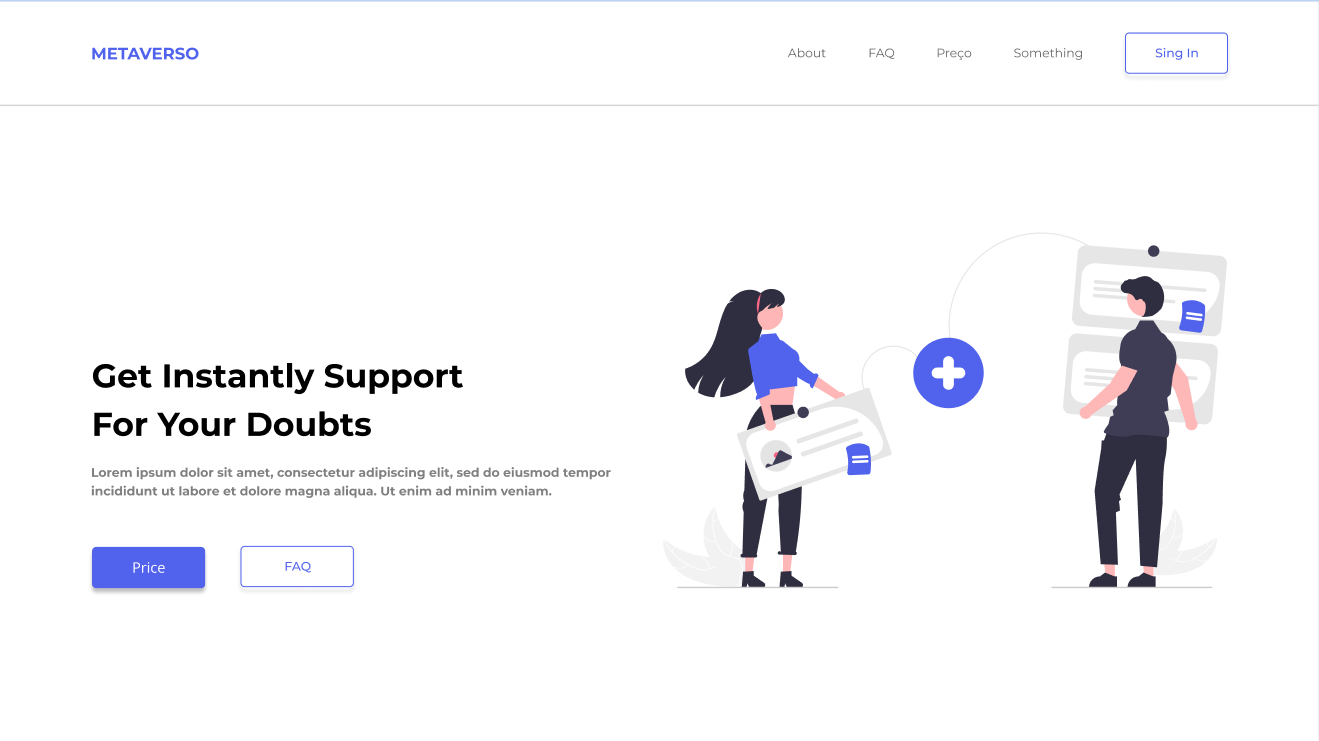
\includegraphics[width=15cm]{LaTeX/metaversoIFSP/anexos/about-section.png} % leia abaixo
        \fonte{Os autores}
    \end{figure}
    
\subsection{FAQ}
    A segunda seção da nossa página principal, será o nosso produto FAQ(gratuito), conforme a \autoref{lp-faq}.
 
    \begin{figure}[!h]
        \caption{FAQ}
        \centering % para centralizarmos a figura
        \label{lp-faq}
        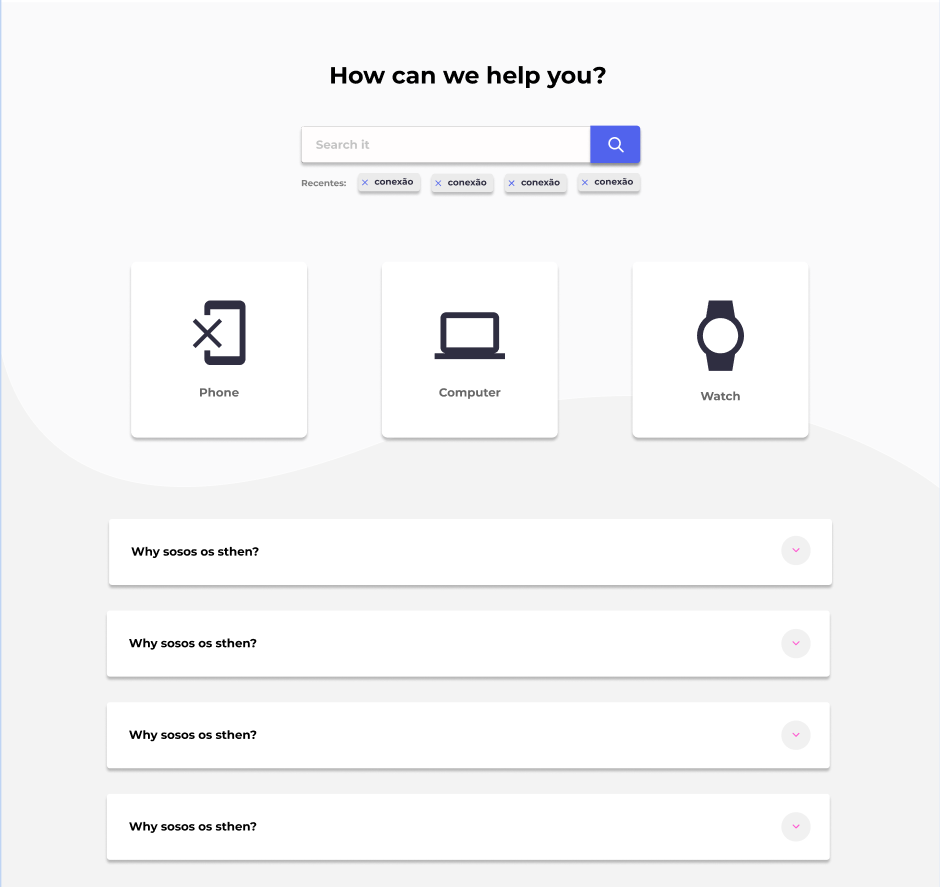
\includegraphics[width=15cm]{LaTeX/metaversoIFSP/anexos/faq.png} % leia abaixo
        \fonte{Os autores}
    \end{figure}
\newpage
\subsection{Planos} 
    A \autoref{lp-planos} apresenta a tela de pricing, na qual trazemos as opções disponíveis dos planos da nossa plataforma.
    \begin{figure}[!h]
        \caption{Planos}
        \centering % para centralizarmos a figura
        \label{lp-planos}
        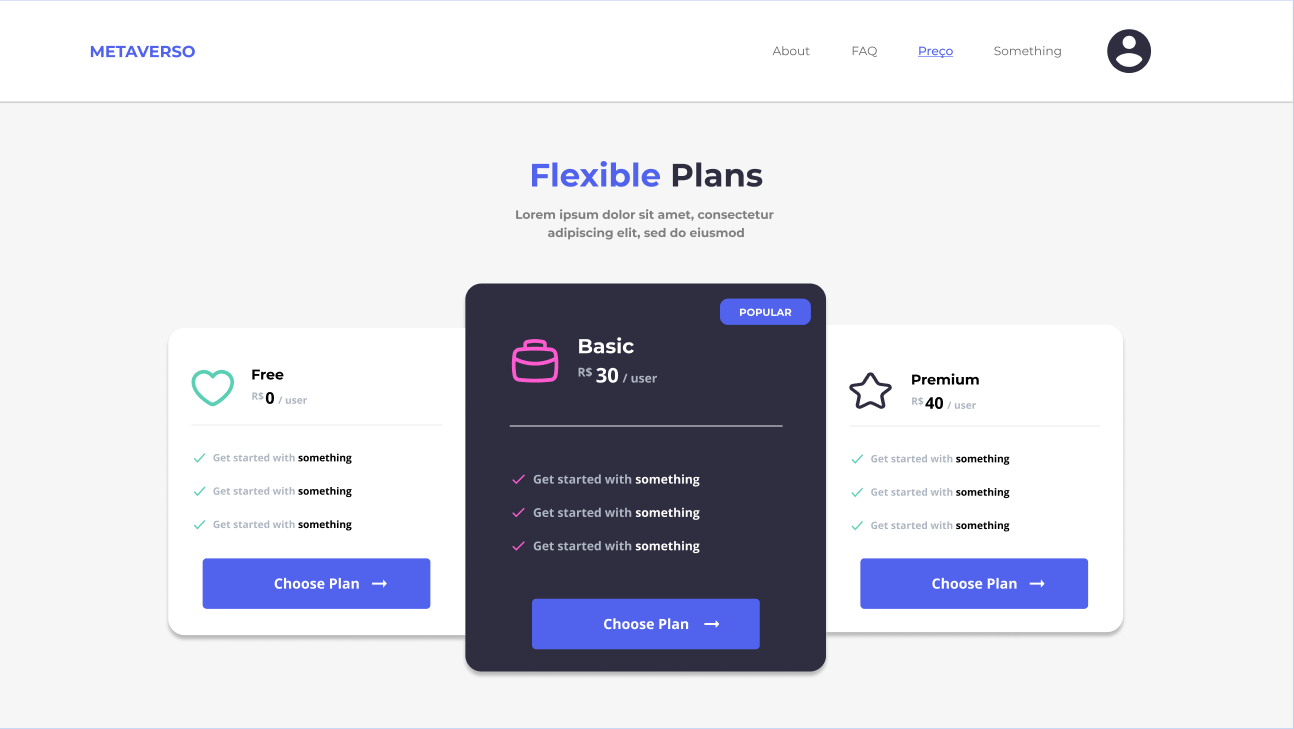
\includegraphics[width=15cm]{LaTeX/metaversoIFSP/anexos/plans.png} % leia abaixo
        \fonte{Os autores}
    \end{figure}
\newpage
\subsection{Login} 
    A \autoref{lp-login} mostra a tela de login, onde o usuário poderá se autenticar para acessar seu portal interno da aplicação.
    \begin{figure}[h]
        \caption{Login}
        \centering % para centralizarmos a figura
        \label{lp-login}
        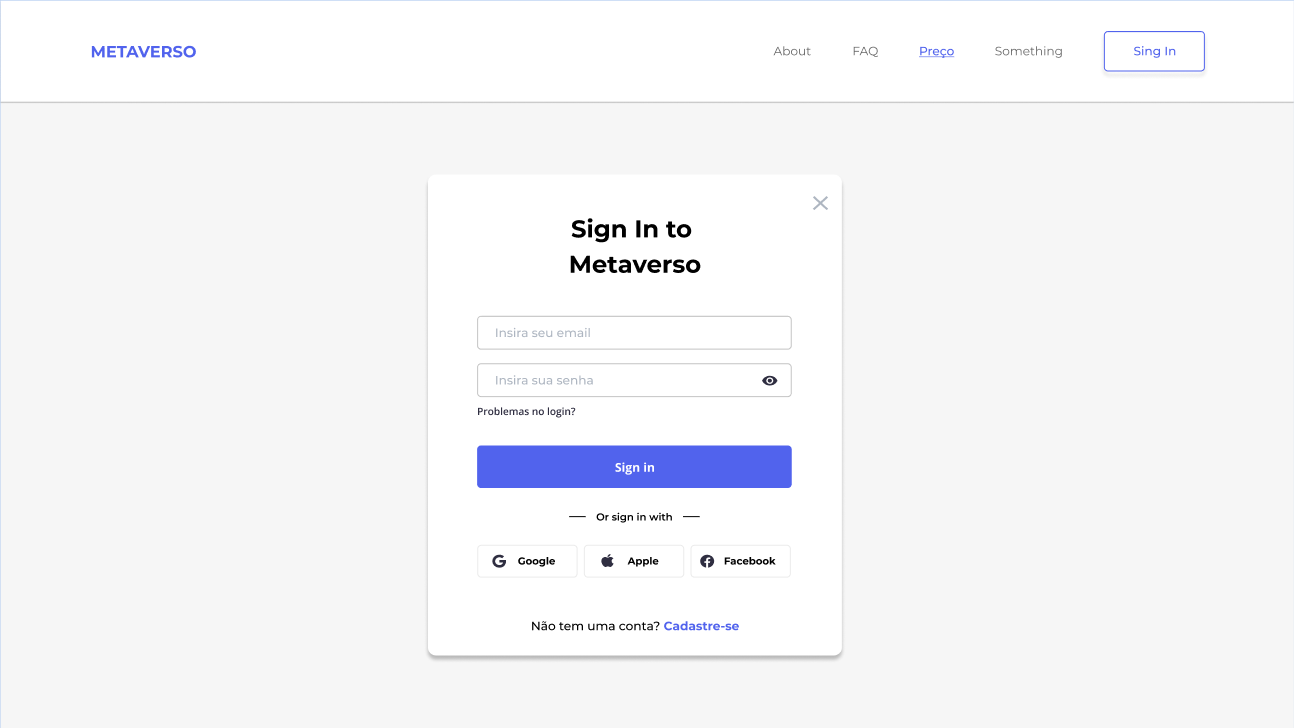
\includegraphics[width=15cm]{LaTeX/metaversoIFSP/anexos/login.png} % leia abaixo
        \fonte{Os autores}
    \end{figure}
    
    
\subsection{Portal (Dashboard)} 
    A \autoref{lp-dashboard} mostra o portal do usuário(Dashboard), focado na tela de chamados do cliente.
    \begin{figure}[h]
        \caption{Portal (Dashboard)}
        \centering % para centralizarmos a figura
        \label{lp-dashboard}
        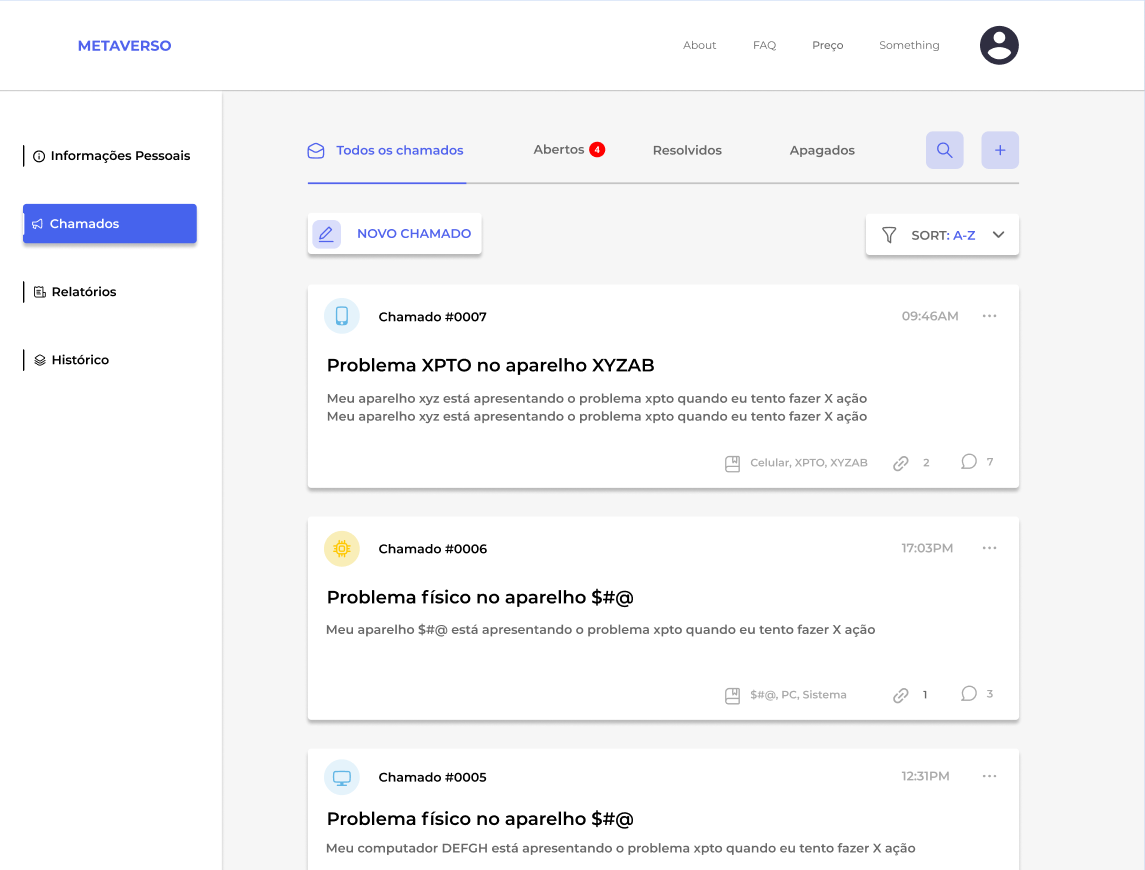
\includegraphics[width=15cm]{LaTeX/metaversoIFSP/anexos/dashboard-chamados.png} % leia abaixo
        \fonte{Os autores}
    \end{figure}
    
\subsection{Novo Chamado} 
        A \autoref{lp-novo-chamado} apresenta o modal com formulário para abertura de novos chamados pelo usuário final.
    \begin{figure}[h]
        \caption{Novo Chamado}
        \centering % para centralizarmos a figura
        \label{lp-novo-chamado}
        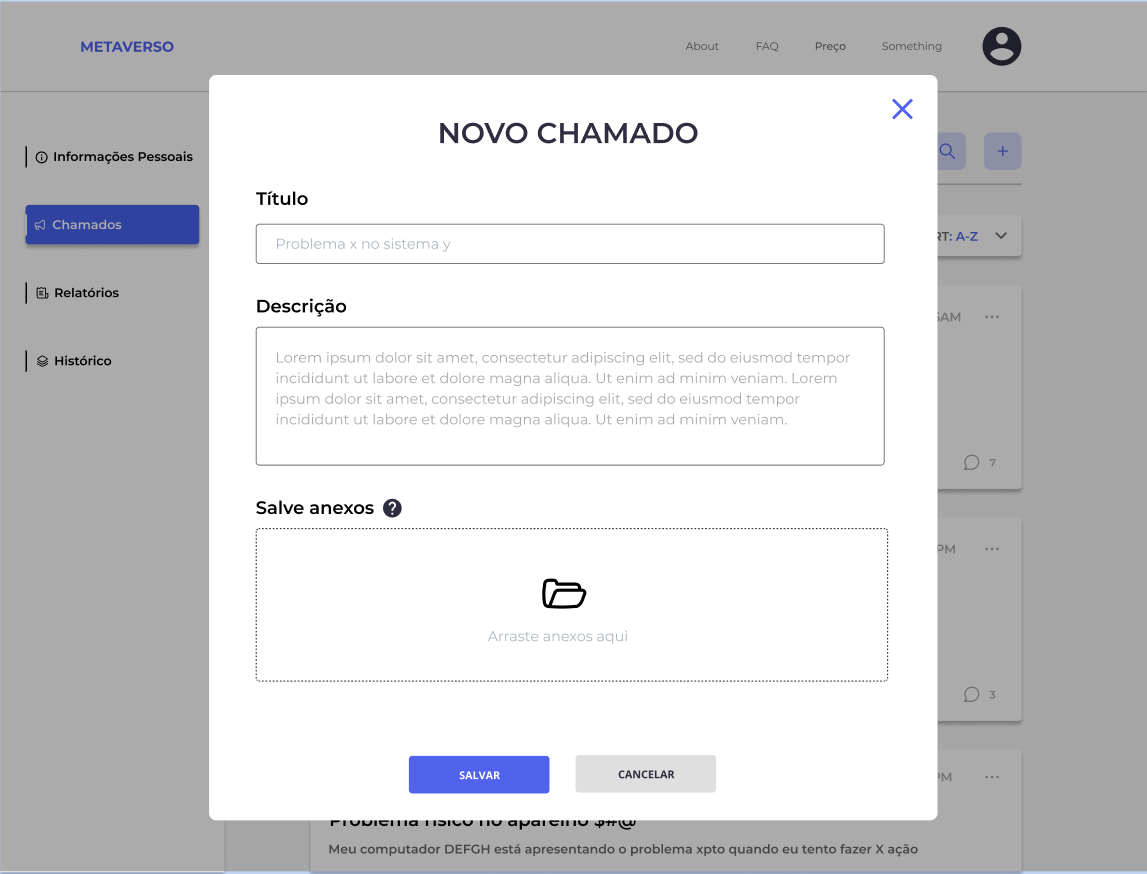
\includegraphics[width=15cm]{LaTeX/metaversoIFSP/anexos/novo-chamado.png} % leia abaixo
        \fonte{Os autores}
    \end{figure}
%	\section{Avaliação SSL}
%	\section{Análise de resposta HTTP}
%	\section{Análise HTML}
%	\section{Métricas do Projeto}
%	\section{Escolhas e Descartes}
%	\subsection{Funcionalidades descartadas}
%	\subsection{Mudanças na infraestrutura}
%	\section{Problemas enfrentados}
	
%	\section{Estatísticas SVN}
	
	\section{Links do Projeto}
	\newcommand{\urlGithub}{https://github.com/MetaversoIFSP/}
	\newcommand{\urlYoutube}{https://www.youtube.com/channel/UCNXlPi5ADeGx1tZbMo_xOqw/}
	\newcommand{\urlSVN}{https://svn.spo.ifsp.edu.br/viewvc/A6PGP/S202201-PI-NOT/Metaverso/}
	\newcommand{\urlBlog}{https://metaversoifsp.blogspot.com/}
	Nesta seção estão disponíveis os \textit{links} de acesso pertinentes ao projeto.
	
    \begin{figure}[h]
        \centering
        \captionsetup{justification=centering}
        \qrcode{\urlGithub}
        \caption{\textit{QR Code} - Repositório remoto GitHub \\ \url{\urlGithub}}
        \fonte{Os autores}
    \end{figure}
    
    \begin{figure}[h]
        \centering
        \captionsetup{justification=centering}
        \qrcode{\urlYoutube}
        \caption{\textit{QR Code} - Canal Metaverso no Youtube \\ \url{\urlYoutube}}
        \fonte{Os autores}
    \end{figure}
    
    \begin{figure}[h]
        \centering
        \captionsetup{justification=centering}
        \qrcode{\urlSVN}
        \caption{\textit{QR Code} - Repositório remoto Subversion\\
        \url{\urlSVN}}
        \fonte{Os autores}
    \end{figure}
    
    \begin{figure}[h]
        \centering
        \captionsetup{justification=centering}
        \qrcode{\urlBlog}
        \caption{\textit{QR Code} - Blog Metaverso \\ \url{\urlBlog}}
        \fonte{Os autores}
    \end{figure}  






% exemplos de escrita LaTeX e erros comuns
\chapter{Exemplos \LaTeX}
\label{cap-exemplos}

\explicacao{ATENÇÃO : Este capítulo e os seguintes demonstram como fazer no {\LaTeX} portanto devem ser lidos em conjunto com o código fonte desse documento}

% exemplo de como inserir uma referencia adicional no sumario (normalmente não utilizado em um trabalho acadêmico)
\addcontentsline{toc}{chapter}{Exemplos que devem ser lidos (mas esse tipo de indicação não vai em um trabalho acadêmico) :-)}

Esse capítulo tem exemplos de escrita utilizando o {\LaTeX}  utilizando \abnTeX, é muito simples escrever em \textbf{negrito}, \textit{itálico} \footnote{apesar de que nesse documento \mostraComandoLaTeX{textit} \mostraComandoLaTeX{emph} tem comportamento parecido é recomendável utilizar \mostraComandoLaTeX{textit} de forma genérica para itálico}, ....


Existem diversos tutoriais para uso de \LaTeX, se você está utilizando esse modelo não precisará se preocupar com muitos dos detalhes técnicos do \LaTeX \space e cuidar somente do seu texto.

Escolha seu editor : \url{https://en.wikipedia.org/wiki/Comparison\_of\_TeX\_editors}, apesar do overleaf sem bem prático, nem todas as funções estão disponíveis na versão gratuita e você pode instalar gratuitamente em seu computador um compilador \LaTeX \space e utilizar um sistema de controle de versão para gerenciar seu documento.


\section{Normas ABNT}

Esse documento modelo já resolve boa parte da padronização NBR 14.724:2011 \cite{NBR14724:2011} que deve ser seguida e inclusive alguns pontos que não são claros pelo modelo de padronização do \ac{ifsp}.

Leia os documentos do {\abnTeX} e do \ac{ifsp}:
\begin{itemize}
    \item \url{https://www.abntex.net.br/}
    
    \item \acs{faq} : \url{https://github.com/abntex/abntex2/wiki/FAQ}
    
    \item \url{http://mirror.unl.edu/ctan/macros/latex/contrib/abntex2/doc/abntex2.pdf}
    
    \item \waUrl{https://spo.ifsp.edu.br/biblioteca?id=184}
\end{itemize}

No \ac{ifsp} você pode acessar todas as normas \ac{abnt} sem custo, as informações estão disponíveis no endereço \waUrl{https://www.ifsp.edu.br/index.php/outras-noticias/52-reitoria/2329-alunos-e-servidores-do-ifsp-podem-acessar-abnt-via-web.html}.

Apesar de alguns elementos serem opcionais na \ac{abnt} eles foram definidos como obrigatórios (folha de rosto, resumo, lista de siglas, lista de ilustrações, glossário etc), nos trabalhos completos de projetos de informática do \ac{ifsp} campus São Paulo. Documentos menores como propostas de projeto, documento de \ac{poc} não necessitam desses elementos, mas alguns podem ser uteis para ajudar no estudo do {\LaTeX} em preparação para o documento final.

\begin{itemize}
    \item Logotipo da instituição, não é citado na \ac{abnt} nem no manual de normalização do \ac{ifsp}, mas aparece em uma imagem do documento de normalização, foi definido que não deve ser incluído na capa;
    
    \item Nome da instituição que é opcional na capa, deve ser utilizado;
    
\end{itemize}



\section{Detalhes textuais}

O documento é dividido em capítulos, e cada capítulo dividido em seções utilizando o \abnTeX \space você pode dividir seus documentos nos níveis de acordo com os comandos:

\begin{itemize}
    \item \mostraComandoLaTeX{chapter}  (1);
    
    \item \mostraComandoLaTeX{section} (1.1);
    
    \item \mostraComandoLaTeX{subsection} (1.1.1);
    
    \item \mostraComandoLaTeX{subsubsection} (1.1.1.1);
    
    \item \mostraComandoLaTeX{subsubsubsection} (1.1.1.1.1).
    
\end{itemize}

Tenha em mente que normalmente se utiliza no máximo o nível \mostraComandoLaTeX{subsection}.
Ao definir as divisões do seu trabalho utilizando as diretivas do \LaTeX, elas são automaticamente inseridas no sumário do documento.


\subsection{Caracteres Reservados e auxiliares}



Alguns caracteres são reservados no \LaTeX \space e por isso para utilizar esses caracteres é necessário utilizar uma forma diferenciada de escrita. É possível utilizar a macro \mostraComandoLaTeX{symbol} com o código \ac{ascii} do caracter desejado, veja no código fonte desse texto como utilizar corretamente esses itens.


\begin{itemize}
\item barra invertida : \textbackslash   \symbol{92}    $\backslash$;
\item til  :  \symbol{126} ;
\item cifrão : \$;
\item sublinhado, \textit{underscore}, \textit{underline} : \_;
\item \enquote{aspas} as macros \mostraComandoLaTeX{enquote} / \mostraComandoLaTeX{textquote} garantem o espaçamento correto, se utilizar diretamente as ASPAS o espaçamento é perdido;
% https://tex.stackexchange.com/questions/80395/no-space-after-closing-double-quote
\item marcadores : \cmark\ \xmark\ \circlemark\ \ding{100} \ - ver mais no \refanexo{pifont-quickref};
\item chaves : \} \{.
\end{itemize}

\subsection{Listas}

Em uma lista de itens cada item deve ser terminado por ponto e virgula, exceto o ultimo item que deve ter um ponto final.

\begin{itemize}
\item item 1;
\item item 2;
\item item ..;
\item item final.
\end{itemize}


\subsection{Citações / Referências}
\label{referencias}

Em um trabalho acadêmico você deve buscar referencias que servem de base para seus estudos, essas referencias devem ser confiáveis, normalmente artigos e livros são confiáveis pois passam por um processo de revisão por especialistas na área. É importante buscar as referencias primárias e não utilizar a informação escrita por outra pessoa (referencia secundária). As citações são definidas pela \citetitle{NBR10520:2002} e as referencias pela \citetitle{NBR6023:2018}, sendo interessante observar que a \citeonline{NBR6023:2018_alteracoes} fez uma resumo com algumas das mudanças ocorridas em 2018.


A \ac{abnt} define a citação da citação (\textit{apud}), mas sua utilização não deve ser feita exceto em casos onde o documento original não possa ser acessado de nenhuma forma. Atualmente a maioria dos documentos se encontra disponível de forma digital o que permite a busca das informações em suas fontes primárias de forma que o \textit{apud} não é bem visto. 

Não é indicada a utilização de sites como Wikipedia como fonte de informações pois a Wikipedia é uma referencia secundária, já que exige que seus artigos tenham referencias da informação, e com isso a utilização da Wikipedia cai no mesmo caso da utilização de \textit{apud} indicada anteriormente, já que é possível buscar a informação diretamente na fonte primária.

Quando for necessário citar sites deve ser utilizada a ferramenta \url{https://web.archive.org}, caso não exista uma referencia salva anteriormente basta salvar e utilizar. O uso dessa ferramenta muitas vezes ajuda também a determinar a data estimada de publicação de informação quando o site já foi salvo anteriormente e não possui data de publicação disponível.



Existem diversas formas de citação que devem ser escolhidas de acordo com o contexto do texto onde são utilizadas, observe os exemplos :

\begin{itemize}
    \item \mostraComandoLaTeX{cite} - utilizada normalmente em final de paragrafo: \newline
    \cite{UML:JACOBSON} | \cite{POWELL:2006} \\ 
        \cite{SCRUMGUIDE:2013} | \cite{urani1994} |\\
        \cite{ETAL5} | \cite{ETAL4}; 
    
    \explicacao{Se as duas ultimas referencias aparecem somente com um autor, você está compilando o documento com uma versão antiga do \mostraPacoteLaTeX{abntexcite}, o overleaf em 2021-07-06 estava desatualizado}
    \explicacao{ABNT 6023:2018 8.1.1.2 recomenda para utilizar TODOS autores sempre, mas permite utilizar et al, dependendo da versão do \mostraPacoteLaTeX{abntexcite} isso não está acontecendo corretamente}

    \item \mostraComandoLaTeX{citeonline}  - utilizada normalmente em textos como \enquote{(segundo|de acordo| com) ...}: \newline
    \citeonline{UML:JACOBSON} | \citeonline{POWELL:2006} \\
        \citeonline{SCRUMGUIDE:2013} | \citeonline{urani1994} \\
        \citeonline{ETAL5} | \citeonline{ETAL4};

    \item \mostraComandoLaTeX{citeauthoronline} - raramente utilizado, quando se deseja citar somente o autor: \newline
    \citeauthoronline{UML:JACOBSON}| \citeauthoronline{POWELL:2006} \\
        \citeauthoronline{SCRUMGUIDE:2013} | \citeauthoronline{urani1994} \\
        \citeauthoronline{ETAL5} | \citeauthoronline{ETAL4};

    \item \mostraComandoLaTeX{citeauthor} - muito pouco utilizado: \newline \citeauthor{UML:JACOBSON}| \citeauthor{POWELL:2006} \\
        \citeauthor{SCRUMGUIDE:2013}| \citeauthor{urani1994} \\
        \citeauthor{ETAL5} | \citeauthor{ETAL4};
    
    \explicacao{Se as duas ultimas referencias aparecem somente com um autor, você está compilando o documento com uma versão antiga do \mostraPacoteLaTeX{abntexcite}, o overleaf em 2021-07-06 estava desatualizado}

    \item \mostraComandoLaTeX{citetitle} - muito pouco utilizado: \newline
    \citetitle{UML:JACOBSON}|\citetitle{POWELL:2006} \\
        \citetitle{SCRUMGUIDE:2013}| \citetitle{urani1994} 
        
    \explicacao{O comando \mostraComandoLaTeX{citetitle} está disponível utilizando a biblioteca \mostraPacoteLaTeX{biblatex}}

\end{itemize}

A documentação do abntex2cite possui muitos exemplos de como utilizar corretamente cada formato de citação : \url{https://mirrors.ibiblio.org/CTAN/macros/latex/contrib/abntex2/doc/abntex2cite-alf.pdf}.

Cada formato de citação deve ser utilizado em um contexto especifico :
\begin{itemize}
    \item De acordo com \citeonline{SCRUMGUIDE:2013} .....;
    
    \item Fonte: \citeonline{SCRUMGUIDE:2013};
    
    \item sua explicação de um assunto baseado em uma referência \cite{SCRUMGUIDE:2013}.
    
\end{itemize}

ATENÇÃO : Alguns parâmetros de formatação foram alterados em 2018, mas não foram corrigidos ainda nos pacotes do \ac{abntex}, devem ser alterados manualmente ou utilizar as versões de desenvolvimento
\begin{itemize}
    \item \url{https://github.com/abntex/abntex2/issues/210}
    
    \item \url{https://github.com/abntex/biblatex-abnt/issues/42}
\end{itemize}

Os dados devem ser definidos corretamente nos arquivos \textquote{.bib} para a correta formatação no texto e na lista de referências.

Para autor com diversas publicações no mesmo ano : são geradas letras automaticamente pelo compilador de acordo com a ordem que são apresentadas na bibliografia, a letra não aparece na lista de referencias. \footnote{\url{https://github.com/abntex/biblatex-abnt/issues/20}}




\subsection{Abreviaturas / Siglas / Glossário}
\label{siglas-glossario}

Palavras que devem ser apresentadas no glossário devem ser citadas especificamente no texto utilizando os comandos de glossário como : \gls{tag}. Nesse modelo as definições de glossário devem ser feitas no arquivo \textbf{defs-glossario.tex}.

As abreviaturas nesse modelo devem ser feitas no arquivo \textbf{defs-siglas.tex}, tomando o cuidado de definir corretamente as siglas de outras línguas e as da língua portuguesa. Abreviaturas normalmente são referenciadas utilizando \mostraComandoLaTeX{ac}, mas podem ser referenciadas diretamente na versão reduzida \textquote{\acs{ifsp}} (\mostraComandoLaTeX{acs}) \space  
ou longa \textquote{\acl{ifsp}} (\mostraComandoLaTeX{acl}).

Na primeira vez que a sigla aparecer no texto o compilador {\LaTeX} mostra por extenso e a partir dai mostra somente a sigla:

\begin{itemize}
    \item \ac{se}
    
    \item \ac{se}
    
\end{itemize}

Quando uma sigla é utilizada em titulo de figura ela não deve aparecer por extenso. A maneira correta para que isso aconteça é utilizar a sigla com \mostraComandoLaTeX{acs} no titulo da figura como apresentado na \autoref{fig_sge1} pela sigla \ac{sge1}.

\begin{figure}[hb]
    \centering
	\caption{\label{fig_sge1}Exemplo de sigla em titulo de ilustração \acs{sge1}}
    \missingfigure[figwidth=6cm]{Exemplo para uso de sigla em titulo \ldots}	
	\fonte{Os autores.}
\end{figure}



Lembre que o {\LaTeX} tem vários passos de compilação, sempre que alterar as chamadas de siglas / referencias é recomendável uma compilação completa do documento.








\subsection{Elementos não textuais / Ilustrações}
\label{elementos-nao-textuais}

Elementos não textuais são aqueles que auxiliam o entendimento, não podem ficar \enquote{jogados} no texto, devem ser citados, cada elemento deve ser identificado por um \mostraComandoLaTeX{label} único que permite a sua referencia, no texto utilizando \mostraComandoLaTeX{ref} ou \mostraComandoLaTeX{autoref}, esses elementos quando definidos corretamente também são inseridos nas listas presentes antes do sumário.

Cuidado com o artigo \textbf{O/A} antes da Figura, Tabela ou Quadro referenciado, deve ser compatível com o tipo da ilustração.

Lembre que o \LaTeX \  vai posicionar os elementos  da melhor maneira possível dentro do documento, sempre faça as referencias utilizando os comandos específicos, nunca utiliza \enquote{acima}, \enquote{"baixo}, \enquote{a seguir}, etc... 

O posicionamento desses elementos é feito pelas rotinas do pacote float, leia a documentação em  \url{http://linorg.usp.br/CTAN/macros/latex/contrib/float/float.pdf}. É recomendável utilizar as opções de posicionamento \textbf{htb}, a opção \textbf{H} deverá ser utilizada somente como ultima alternativa de posicionamento e em alguns casos a utilização de \mostraComandoLaTeX{FloatBarrier} pode também melhorar o resultado se utilizada com cuidado.

Lembre que se houver uma grande distancia entre a ilustração no documento \ac{pdf} e sua definição original no documento isso significa que existe muito pouco texto em seu documento e isso não oferece muitas opções para o {\LaTeX} organizar as ilustrações. Você precisa nesse caso melhorar a descrição textual das ilustrações.


Para casos onde existe uma grande distancia entre a ilustração e o ponto de referencia no texto esse modelo possui macros \mostraComandoLaTeX{autorefwithpage} e \mostraComandoLaTeX{autorefwithpagedistance} a primeira sempre indica página onde a ilustração foi colocada e a segunda somente se a ilustração estiver mais distante que o número de páginas indicado como parâmetro, Ex. \autorefwithpage{fig_logo_A3}. Isso deve ser utilizado somente quando existe mais de uma referencia para mesma ilustração e não para deixar a ilustração distante de uma única referencia.

O titulo da ilustração deve ser apresentado sempre no topo (conforme \citetitle{NBR14724:2011}, era na parte inferior na  \citetitle{NBR14724:2005}), e a fonte deve ficar na parte inferior \cite{NBR14724:2011}. A norma não possui um exemplo direto do uso das fontes e é possível encontrar exemplos com e sem ponto final nas fontes das ilustrações. Considerando a utilização de ponto no manual do \ac{ibge} nesse modelo foi escolhido utilizar o ponto final na fonte das ilustrações.





% ---
\subsection{QR-Code}
% ---
\index{qr-code}
\explicacao{Entendam que faz sentido colocar aqui nesse MODELO uma seção chamada QR-Code pois está sendo explicada a forma de utilização, mas em um documento normal onde o QR-Code é utilizado para apresentar uma URL não faz sentido, já que ele é somente uma ferramenta como um gráfico de pizza}


A utilização de códigos \ac{qr} facilita o acesso de endereços da internet a partir de dispositivos móveis com câmera.
As Figuras \ref{qr-url-1} e \ref{qr-url-2} demonstram dois exemplos de endereços apresentados com essa tecnologia.


Para facilitar a utilização dos códigos \ac{qr}, deve-se tomar cuidado para não deixa-los alinhados na vertical se houverem vários seguidos, pois dificulta a seleção a partir da câmera no dispositivo móvel.

Os endereços também devem ter seu \ac{url} apresentada de forma que mesmo um usuário que esteja fazendo a leitura do documento eletrônico também vai conseguir acessar o endereço indicado. Observe que as figuras de demonstração possuem tanto o código \ac{qr} como o \ac{url}.

Um exemplo para utilização de mais códigos de barra pode ser visto em : \urlmodelo.

Atenção, alguns compiladores podem ter problemas em utilizar a biblioteca \textbf{pstricks} necessária para gerar QR-Codes, no sharelatex em 2017-05 a compilação ocorre perfeitamente utilizando a opção de compilador "XeLatex", ele é mais lento que outras opções.


\begin{figure}[htb]
\caption{\label{qr-url-1}URL para acesso ao documento exemplo}
\begin{pspicture}(25mm,25mm)
\psbarcode{\urlmodelosimples}{eclevel=H width=1.0 height=1.0}{qrcode}
\end{pspicture}
\legend{\urlmodelo}
\fonte{Os Autores.}
\end{figure}


\explicacao{o repositório indicado pela \autoref{qr-url-2} não está sendo atualizado, utilize a versão disponível no overleaf}

% colocando figura qrcode na direita para facilitar o uso da camera deixando cada qrcode em um alinhamento diferente
% se deixar os dois qrcodes um em cima do outro dificulta acessar o desejado
\begin{figure}[htb]
\caption{\label{qr-url-2}Repositório original de classes IFSP \LaTeX}
\begin{flushright}
\begin{pspicture}(25mm,25mm)
\psbarcode{https://github.com/ivanfmartinez/latexlib/tree/master/ifsp}{eclevel=H width=1.0 height=1.0}{qrcode}
\end{pspicture}
\legend{\url{https://github.com/ivanfmartinez/latexlib/tree/master/ifsp}}
\fonte{Os Autores.}
\end{flushright}

\end{figure}


\subsection{Organizando pendências}

Durante o desenvolvimento de um trabalho escrito é normal que alguns elementos sejam gerados posteriormente, mas é importante se organizar para não esquecer de fazer os ajustes necessários. Para isso recomendo a utilização do pacote \textbf{todonotes} que oferece diversos recursos para gerar lembretes das pendencias. O manual do \textbf{todonotes} está disponível no \autoref{manual-todonotes}\footnote{observe que existe um erro nesse documento, já que a referencia deveria ser Anexo e aparece como Apêndice,  existe um \textit{bug} no abntex2 ao referenciar anexos, para fazer corretamente veja \url{https://github.com/abntex/abntex2/issues/76} e utilize \mostraComandoLaTeX{refanexo} que está disponível nesse modelo.}.

É possível fazer anotações de pendencias inclusive indicando as pessoas responsáveis por elas, % nao mover o todo pois foi feito no meio do paragrafo exatamente para demonstrar um possível problema de formato
\todo[inline,author=Pessoa1]{fazer revisão das imagens do texto} e para facilitar a visualização criar imagens que funcionam como marcadores para figuras que serão incluídas posteriormente.

Cuidado ao utilizar as anotações \textit{inline} pois o texto ficara quebrado, como no paragrafo anterior.


\begin{figure}[htb]
    \centering
	\caption{\label{fig_todo1}Imagem que ainda não foi gerada}
	\missingfigure[figwidth=10cm]{você está atrasado pois ainda não criou esta figura}
	\fonte{dados do Projeto.}
\end{figure}



\subsection{Tabelas e Quadros}
\label{tabelas-e-quadros}
Quadros e Tabelas são informações tabulares, mas Tabelas tem como objetivo apresentar números. A ‘norma’ 14724 \cite[3.32]{NBR14724:2011} define a Tabela como sendo uma \enquote{forma não discursiva de apresentar informações das quais o dado numérico se destaca como informação central} e que devem seguir padronização do \ac{ibge}  \cite[5.9]{NBR14724:2011}. O \ac{ibge} padronizou a apresentações de dados tabulares em 1993 \cite{tabular-ibge}.

Informações adicionais sobre o de tabelas no {\LaTeX} podem ser obtidas em  \url{https://en.wikibooks.org/wiki/LaTeX/Tables}.

Antes de utilizar \index{longtable}\textbf{longtable} procure reorganizar o seu layout ou quebrar manualmente em múltiplos quadros / tabelas, pois isso ainda facilita a compreensão pelo leitor.

% https://biblioteca.ibge.gov.br/visualizacao/livros/liv23907.pdf

\index{quadros}O \autoref{quadro-exemplo} é um exemplo de dados tabulares gerados em 
\LaTeX.



\begin{quadro}[htb]
\centering
\ABNTEXfontereduzida
\caption[Níveis de investigação]{Níveis de investigação}
\label{quadro-exemplo}
\begin{tabular}{|p{2.6cm}|p{6.0cm}|p{2.25cm}|p{3.40cm}|}
  \hline
   \thead{Nível de\\Investigação} & \thead{Insumos}  & \thead{Sistemas de\\ Investigação}  & \thead{Produtos}  \\
    \hline
    Meta-nível & Filosofia\index{filosofia} da Ciência  & Epistemologia &
    Paradigma  \\
    \hline
    Nível do objeto & Paradigmas do metanível e evidências do nível inferior &
    Ciência  & Teorias e modelos \\
    \hline
    Nível inferior & Modelos e métodos do nível do objeto e problemas do nível inferior & Prática & Solução de problemas  \\
   \hline
\end{tabular}
\fonte{O Autor.}
\end{quadro}



\index{tabelas}Já a \autoref{tab-exemplo} foi criada conforme o padrão \citeonline{tabular-ibge} requerido pelas normas da \ac{abnt} para documentos técnicos e acadêmicos. Observe que não existem bordas laterais e nem linhas separadoras em uma Tabela e as colunas numéricas tem alinhamento à direita. 

\begin{table}[htb]
\centering
\caption{Métricas de desenvolvimento}
\label{tab-exemplo}
\begin{tabular}{p{2.6cm}rrr}
    \hline
   \thead{Item} & \thead{Janeiro}  & \thead{Fevereiro}  & \thead{Março}  \\
    \hline
    Classes & 2  & 10 & 20  \\
    Linhas & 100  & 250 & 543 \\
    \hline
\end{tabular}
\fonte{Os autores.}
\end{table}

\def\equationautorefname~#1\null{%
  Equação~(#1)\null
}


Para facilitar a criação de tabelas e quadros existem algumas ferramentas como o Tables Generator \url{http://www.tablesgenerator.com/latex_tables} que permite a criação de forma visual gerando o código \LaTeX\ correspondente. E o site \url{https://www.latex-tables.com/} permite converter planilhas em código \LaTeX.


\index{equação}\index{Pitágoras}A \autoref{eq-pythagoras} demonstra que também é possível escrever equações diretamente em \LaTeX

\begin{equation}\label{eq-pythagoras}
a^2+b^2=c^2\,.
\end{equation}






% ---
\subsection{Figuras}
\label{sec_figuras}
% ---

\index{figuras}Figuras podem ser criadas diretamente em \LaTeX,
como o exemplo da \autoref{fig_circulo}, ou inseridas a partir de arquivos externos como a \autoref{fig_logo}, que é o Logotipo do \ac{ifsp}. \index{logotipo}

% Aqui foi utilizada uma figura unica para demostrar a diferença de qualidade entr e vetorizado e não vetorizado pois fica mais simples, já que cada leitor pode ver esse documento em monitores com diferentes qualidades...
As figuras externas devem possuir boa qualidade e preferencialmente serem vetorizadas para se obter o melhor resultado. A \autoref{fig:nao_vetorizado_e_vetorizado} apresenta duas versões de uma mesma imagem demonstrando a variação de qualidade que pode acontecer quando não for utilizada a versão vetorizada, quando a figura possui elementos textuais pode até inviabilizar a leitura. As Figuras \ref{fig:uml_dia_nao_vetorizado_jpeg}, \ref{fig:uml_dia_vetorizado_eps} e \ref{fig:uml_dia_vetorizado_svg} foram reduzidas propositalmente no documento para demonstrar a diferença entre os formatos de arquivo. A diferença fica mais perceptível quando o documento é impresso ou quando existem textos pequenos e é necessário fazer zoom para visualização.

Procure criar suas imagens e diagramas pensando em utilizar impressão em preto-e-branco ou escala de cinza. Isto é importante, principalmente quando se pretende publicar o trabalho, uma vez que a maioria das publicações são somente em preto-e-branco. Outro benefício é o custo de impressão, normalmente menor para páginas preto-e-branco em relação a páginas coloridas.

Para diagramas em \ac{uml} o PlantUML pode ser utilizado para gerar código {\LaTeX} como exemplo na  \autoref{diagramauml}.


Se não houver a possibilidade de utilização de uma imagem vetorizada e existem diversos detalhes utilize \ac{png} em vez de \gls{jpg} ou outros formatos de menor qualidade, observe as diferenças nos exemplos apresentados em :  \waUrlTitle{https://tex.stackexchange.com/questions/136087/selecting-best-file-extension-for-graphics-figures-pictures}{Selecting best file extension for graphics figures pictures}.


\begin{figure}[htb]
	\caption{\label{fig_circulo}A delimitação do espaço}
	\begin{center}
	    \setlength{\unitlength}{5cm}
		\begin{picture}(1,1)
		\put(0,0){\line(0,1){1}}
		\put(0,0){\line(1,0){1}}
		\put(0,0){\line(1,1){1}}
		\put(0,0){\line(1,2){.5}}
		\put(0,0){\line(1,3){.3333}}
		\put(0,0){\line(1,4){.25}}
		\put(0,0){\line(1,5){.2}}
		\put(0,0){\line(1,6){.1667}}
		\put(0,0){\line(2,1){1}}
		\put(0,0){\line(2,3){.6667}}
		\put(0,0){\line(2,5){.4}}
		\put(0,0){\line(3,1){1}}
		\put(0,0){\line(3,2){1}}
		\put(0,0){\line(3,4){.75}}
		\put(0,0){\line(3,5){.6}}
		\put(0,0){\line(4,1){1}}
		\put(0,0){\line(4,3){1}}
		\put(0,0){\line(4,5){.8}}
		\put(0,0){\line(5,1){1}}
		\put(0,0){\line(5,2){1}}
		\put(0,0){\line(5,3){1}}
		\put(0,0){\line(5,4){1}}
		\put(0,0){\line(5,6){.8333}}
		\put(0,0){\line(6,1){1}}
		\put(0,0){\line(6,5){1}}
		\end{picture}
	\end{center}
	\fonte{Modelo Canônico ABNTeX2.}
\end{figure}


\begin{figure}[htb]
    \centering
	\caption{\label{fig_logo}Logotipo \ac{ifsp}}
	\includegraphics{\ifspprefixo/logo-02.jpg}
	\fonte{\ac{ifsp}.}
\end{figure}

\begin{figure}
    \centering
    \caption{Exemplo de imagem não vetorizada e vetorizada}
    \label{fig:nao_vetorizado_e_vetorizado}
	\includegraphics[width=0.95\textwidth]{erros/exemploVetorizacao.png}
    \fonte{\citeonline{vetorizacao}.}
\end{figure}
    

% Essas imagens foram reduzidas na apresentação para demonstrar o efeito da alteração de escala em imagens não vetorizadas
\begin{figure}
    \centering
    \caption{Exemplo de diagrama - salvo em imagem não vetorizada - JPEG}
    \label{fig:uml_dia_nao_vetorizado_jpeg}
	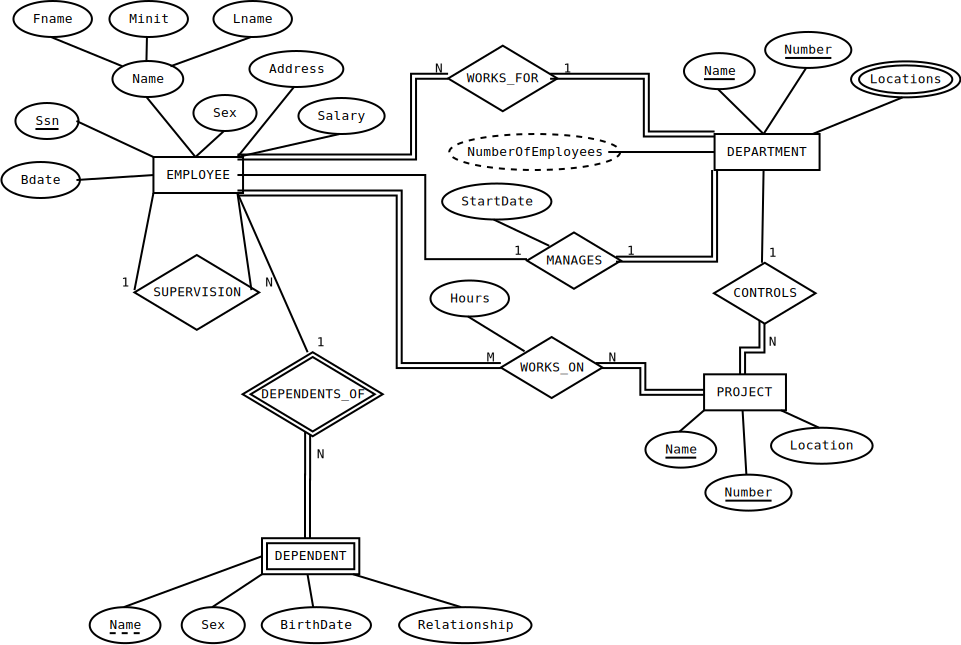
\includegraphics[width=0.6\textwidth]{exemplos/diagramas/ER.jpeg}
    \fonte{Indicar autor original.}
\end{figure}


\begin{figure}
    \centering
    \caption{Exemplo de diagrama - salvo imagem vetorizada - EPS}
    \label{fig:uml_dia_vetorizado_eps}
	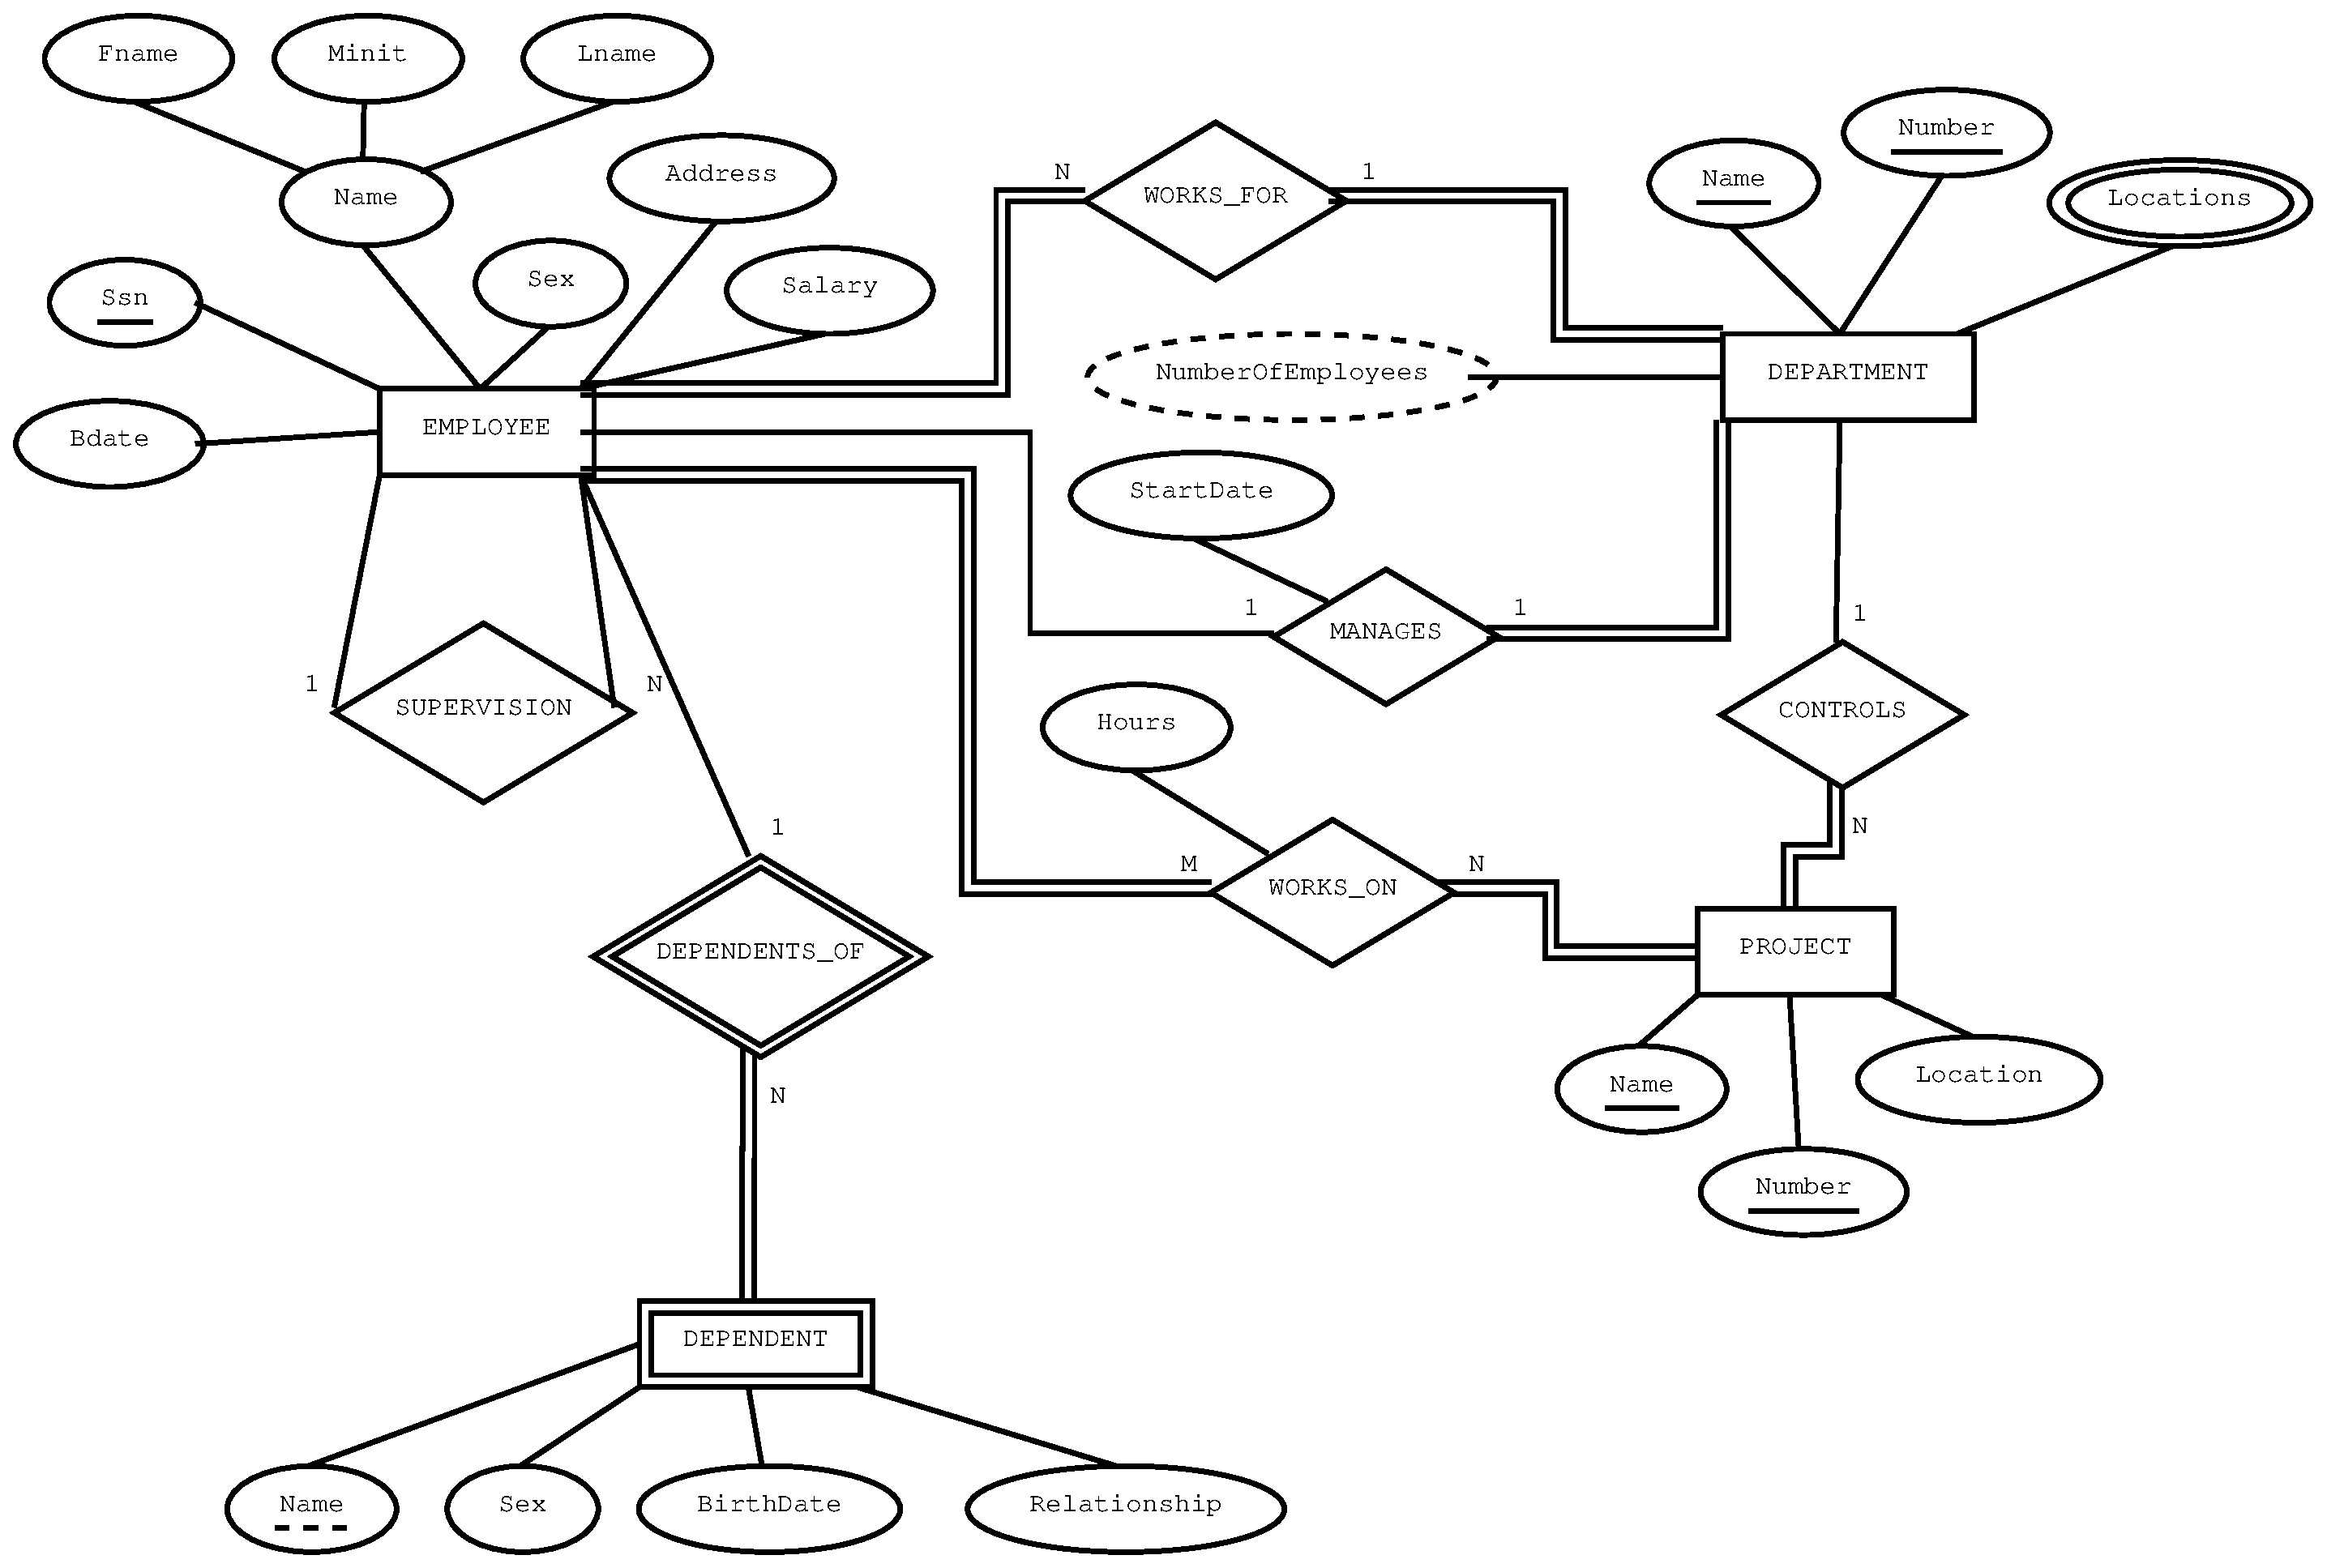
\includegraphics[width=0.6\textwidth]{exemplos/diagramas/ER.eps}
    \fonte{Indicar autor original.}
\end{figure}

\begin{figure}
    \centering
    \caption{Exemplo de diagrama - salvo imagem vetorizada - SVG}
    \label{fig:uml_dia_vetorizado_svg}
    \includesvg[inkscapelatex=false,width=0.6\textwidth]{exemplos/diagramas/ER.svg}
    \fonte{Indicar autor original.}
\end{figure}



% generated by Plantuml 7997beta
\definecolor{plantucolor0000}{RGB}{254,254,206}
\definecolor{plantucolor0001}{RGB}{168,0,54}
\definecolor{plantucolor0002}{RGB}{173,209,178}
\definecolor{plantucolor0003}{RGB}{0,0,0}
\definecolor{plantucolor0004}{RGB}{0,0,255}

\begin{figure}[htb]
    \centering
    \caption{\label{diagramauml}Exemplo de Diagrama UML gerado a partir do PlantUML}
\begin{tikzpicture}[yscale=-1]
\draw[color=plantucolor0001,fill=plantucolor0000,line width=1.5pt] (131pt,29pt) rectangle (223pt,90.8359pt);
\draw[color=plantucolor0001,fill=plantucolor0002,line width=1.0pt] (146pt,45pt) ellipse (11pt and 11pt);
\draw[color=black,fill=black] (148.7656pt,40.875pt) ..controls (148.9219pt,40.6563pt) .. (149.1094pt,40.5469pt) ..controls (149.2969pt,40.4375pt) .. (149.5156pt,40.4375pt) ..controls (149.8906pt,40.4375pt) .. (150.125pt,40.6953pt) ..controls (150.3594pt,40.9531pt) .. (150.3594pt,41.5625pt) -- (150.3594pt,43.0156pt) ..controls (150.3594pt,43.625pt) .. (150.125pt,43.8906pt) ..controls (149.8906pt,44.1563pt) .. (149.5156pt,44.1563pt) ..controls (149.1719pt,44.1563pt) .. (148.9688pt,43.9531pt) ..controls (148.7656pt,43.7656pt) .. (148.6563pt,43.25pt) ..controls (148.6094pt,42.8906pt) .. (148.4219pt,42.7031pt) ..controls (148.0938pt,42.3281pt) .. (147.4844pt,42.1094pt) ..controls (146.875pt,41.8906pt) .. (146.25pt,41.8906pt) ..controls (145.4844pt,41.8906pt) .. (144.8516pt,42.2188pt) ..controls (144.2188pt,42.5469pt) .. (143.7266pt,43.2969pt) ..controls (143.2344pt,44.0469pt) .. (143.2344pt,45.0781pt) -- (143.2344pt,46.1719pt) ..controls (143.2344pt,47.4063pt) .. (144.125pt,48.2266pt) ..controls (145.0156pt,49.0469pt) .. (146.6094pt,49.0469pt) ..controls (147.5469pt,49.0469pt) .. (148.2031pt,48.7969pt) ..controls (148.5938pt,48.6406pt) .. (149.0156pt,48.2031pt) ..controls (149.2813pt,47.9375pt) .. (149.4297pt,47.8594pt) ..controls (149.5781pt,47.7813pt) .. (149.7813pt,47.7813pt) ..controls (150.1094pt,47.7813pt) .. (150.3672pt,48.0391pt) ..controls (150.625pt,48.2969pt) .. (150.625pt,48.6406pt) ..controls (150.625pt,48.9844pt) .. (150.2813pt,49.3906pt) ..controls (149.7813pt,49.9688pt) .. (148.9844pt,50.2969pt) ..controls (147.9063pt,50.75pt) .. (146.6094pt,50.75pt) ..controls (145.0938pt,50.75pt) .. (143.8906pt,50.125pt) ..controls (142.9063pt,49.625pt) .. (142.2188pt,48.5547pt) ..controls (141.5313pt,47.4844pt) .. (141.5313pt,46.2031pt) -- (141.5313pt,45.0469pt) ..controls (141.5313pt,43.7188pt) .. (142.1484pt,42.5703pt) ..controls (142.7656pt,41.4219pt) .. (143.8594pt,40.8047pt) ..controls (144.9531pt,40.1875pt) .. (146.1875pt,40.1875pt) ..controls (146.9219pt,40.1875pt) .. (147.5703pt,40.3516pt) ..controls (148.2188pt,40.5156pt) .. (148.7656pt,40.875pt);
\node at (160pt,37.4531pt)[below right]{Subscriber};
\draw[color=plantucolor0001,line width=1.5pt] (132pt,61pt) -- (222pt,61pt);
\node at (137pt,65pt)[below right]{subscriberId};
\draw[color=plantucolor0001,line width=1.5pt] (132pt,82.8359pt) -- (222pt,82.8359pt);
\draw[color=plantucolor0001,fill=plantucolor0000,line width=1.5pt] (31pt,212pt) rectangle (137pt,273.8359pt);
\draw[color=plantucolor0001,fill=plantucolor0002,line width=1.0pt] (46pt,228pt) ellipse (11pt and 11pt);
\draw[color=black,fill=black] (48.7656pt,223.875pt) ..controls (48.9219pt,223.6563pt) .. (49.1094pt,223.5469pt) ..controls (49.2969pt,223.4375pt) .. (49.5156pt,223.4375pt) ..controls (49.8906pt,223.4375pt) .. (50.125pt,223.6953pt) ..controls (50.3594pt,223.9531pt) .. (50.3594pt,224.5625pt) -- (50.3594pt,226.0156pt) ..controls (50.3594pt,226.625pt) .. (50.125pt,226.8906pt) ..controls (49.8906pt,227.1563pt) .. (49.5156pt,227.1563pt) ..controls (49.1719pt,227.1563pt) .. (48.9688pt,226.9531pt) ..controls (48.7656pt,226.7656pt) .. (48.6563pt,226.25pt) ..controls (48.6094pt,225.8906pt) .. (48.4219pt,225.7031pt) ..controls (48.0938pt,225.3281pt) .. (47.4844pt,225.1094pt) ..controls (46.875pt,224.8906pt) .. (46.25pt,224.8906pt) ..controls (45.4844pt,224.8906pt) .. (44.8516pt,225.2188pt) ..controls (44.2188pt,225.5469pt) .. (43.7266pt,226.2969pt) ..controls (43.2344pt,227.0469pt) .. (43.2344pt,228.0781pt) -- (43.2344pt,229.1719pt) ..controls (43.2344pt,230.4063pt) .. (44.125pt,231.2266pt) ..controls (45.0156pt,232.0469pt) .. (46.6094pt,232.0469pt) ..controls (47.5469pt,232.0469pt) .. (48.2031pt,231.7969pt) ..controls (48.5938pt,231.6406pt) .. (49.0156pt,231.2031pt) ..controls (49.2813pt,230.9375pt) .. (49.4297pt,230.8594pt) ..controls (49.5781pt,230.7813pt) .. (49.7813pt,230.7813pt) ..controls (50.1094pt,230.7813pt) .. (50.3672pt,231.0391pt) ..controls (50.625pt,231.2969pt) .. (50.625pt,231.6406pt) ..controls (50.625pt,231.9844pt) .. (50.2813pt,232.3906pt) ..controls (49.7813pt,232.9688pt) .. (48.9844pt,233.2969pt) ..controls (47.9063pt,233.75pt) .. (46.6094pt,233.75pt) ..controls (45.0938pt,233.75pt) .. (43.8906pt,233.125pt) ..controls (42.9063pt,232.625pt) .. (42.2188pt,231.5547pt) ..controls (41.5313pt,230.4844pt) .. (41.5313pt,229.2031pt) -- (41.5313pt,228.0469pt) ..controls (41.5313pt,226.7188pt) .. (42.1484pt,225.5703pt) ..controls (42.7656pt,224.4219pt) .. (43.8594pt,223.8047pt) ..controls (44.9531pt,223.1875pt) .. (46.1875pt,223.1875pt) ..controls (46.9219pt,223.1875pt) .. (47.5703pt,223.3516pt) ..controls (48.2188pt,223.5156pt) .. (48.7656pt,223.875pt);
\node at (60pt,220.4531pt)[below right]{AccumUsage};
\draw[color=plantucolor0001,line width=1.5pt] (32pt,244pt) -- (136pt,244pt);
\node at (37pt,248pt)[below right]{subscriberId};
\draw[color=plantucolor0001,line width=1.5pt] (32pt,265.8359pt) -- (136pt,265.8359pt);
\draw[color=plantucolor0001,fill=plantucolor0000,line width=1.5pt] (221pt,191pt) rectangle (318pt,294.3438pt);
\draw[color=plantucolor0001,fill=plantucolor0002,line width=1.0pt] (240.05pt,207pt) ellipse (11pt and 11pt);
\draw[color=black,fill=black] (242.8156pt,202.875pt) ..controls (242.9719pt,202.6563pt) .. (243.1594pt,202.5469pt) ..controls (243.3469pt,202.4375pt) .. (243.5656pt,202.4375pt) ..controls (243.9406pt,202.4375pt) .. (244.175pt,202.6953pt) ..controls (244.4094pt,202.9531pt) .. (244.4094pt,203.5625pt) -- (244.4094pt,205.0156pt) ..controls (244.4094pt,205.625pt) .. (244.175pt,205.8906pt) ..controls (243.9406pt,206.1563pt) .. (243.5656pt,206.1563pt) ..controls (243.2219pt,206.1563pt) .. (243.0188pt,205.9531pt) ..controls (242.8156pt,205.7656pt) .. (242.7063pt,205.25pt) ..controls (242.6594pt,204.8906pt) .. (242.4719pt,204.7031pt) ..controls (242.1438pt,204.3281pt) .. (241.5344pt,204.1094pt) ..controls (240.925pt,203.8906pt) .. (240.3pt,203.8906pt) ..controls (239.5344pt,203.8906pt) .. (238.9016pt,204.2188pt) ..controls (238.2688pt,204.5469pt) .. (237.7766pt,205.2969pt) ..controls (237.2844pt,206.0469pt) .. (237.2844pt,207.0781pt) -- (237.2844pt,208.1719pt) ..controls (237.2844pt,209.4063pt) .. (238.175pt,210.2266pt) ..controls (239.0656pt,211.0469pt) .. (240.6594pt,211.0469pt) ..controls (241.5969pt,211.0469pt) .. (242.2531pt,210.7969pt) ..controls (242.6438pt,210.6406pt) .. (243.0656pt,210.2031pt) ..controls (243.3313pt,209.9375pt) .. (243.4797pt,209.8594pt) ..controls (243.6281pt,209.7813pt) .. (243.8313pt,209.7813pt) ..controls (244.1594pt,209.7813pt) .. (244.4172pt,210.0391pt) ..controls (244.675pt,210.2969pt) .. (244.675pt,210.6406pt) ..controls (244.675pt,210.9844pt) .. (244.3313pt,211.3906pt) ..controls (243.8313pt,211.9688pt) .. (243.0344pt,212.2969pt) ..controls (241.9563pt,212.75pt) .. (240.6594pt,212.75pt) ..controls (239.1438pt,212.75pt) .. (237.9406pt,212.125pt) ..controls (236.9563pt,211.625pt) .. (236.2688pt,210.5547pt) ..controls (235.5813pt,209.4844pt) .. (235.5813pt,208.2031pt) -- (235.5813pt,207.0469pt) ..controls (235.5813pt,205.7188pt) .. (236.1984pt,204.5703pt) ..controls (236.8156pt,203.4219pt) .. (237.9094pt,202.8047pt) ..controls (239.0031pt,202.1875pt) .. (240.2375pt,202.1875pt) ..controls (240.9719pt,202.1875pt) .. (241.6203pt,202.3516pt) ..controls (242.2688pt,202.5156pt) .. (242.8156pt,202.875pt);
\node at (254.95pt,199.4531pt)[below right]{IpSession};
\draw[color=plantucolor0001,line width=1.5pt] (222pt,223pt) -- (317pt,223pt);
\node at (227pt,227pt)[below right]{ipAddress};
\node at (227pt,240.8359pt)[below right]{specificData};
\node at (227pt,254.6719pt)[below right]{sapcOriginStateId};
\node at (227pt,268.5078pt)[below right]{apnId};
\draw[color=plantucolor0001,line width=1.5pt] (222pt,286.3438pt) -- (317pt,286.3438pt);
\draw[color=plantucolor0004] (191.942pt,90.081pt) ..controls (205.204pt,115.893pt) and (224.952pt,154.325pt) .. (241.265pt,186.076pt);
\draw[color=plantucolor0004,fill=plantucolor0004] (243.646pt,190.709pt) -- (243.0894pt,180.8759pt) -- (241.3604pt,186.262pt) -- (235.9742pt,184.5329pt) -- (243.646pt,190.709pt) -- cycle;
\node at (191.0584pt,98.9168pt)[below right]{1};
\node at (230.3817pt,166.6703pt)[below right]{1..*};
\draw[color=plantucolor0001] (162.058pt,90.081pt) ..controls (145.645pt,122.023pt) and (119.302pt,173.295pt) .. (101.824pt,207.31pt);
\draw[color=plantucolor0001,fill=plantucolor0001] (99.5252pt,211.784pt) -- (107.1969pt,205.6078pt) -- (101.8108pt,207.337pt) -- (100.0816pt,201.9509pt) -- (99.5252pt,211.784pt) -- cycle;
\node at (143.0082pt,98.7264pt)[below right]{1};
\node at (101.801pt,187.522pt)[below right]{0..1};
\end{tikzpicture}
	\legend{Fonte: Exemplos PlantUML.}
\end{figure}

A \autoref{fig_diag_virado} exemplifica como utilizar uma imagem em formato paisagem (página inteira). Obs: Utilizamos propositalmente uma imagem não vetorizada de forma a ilustrar o procedimento e também para apresentar que a qualidade não fica boa o suficiente para leitura. Uma versão vetorizada dessa figura teria qualidade melhor.


% observe que a imagem a seguir teve que ser ajustada para caber corretamente na página
% por não ser uma imagem vetorizada a qualidade não é a melhor possivel
\begin{sidewaysfigure}[htb]
    \centering
	\caption{\label{fig_diag_virado}Diagrama Virado - Exemplo}
	\includegraphics[width=0.9\textwidth]{exemplos/exemplo_diag_horizontal.png}
	\fonte{\citeonline{openehrCompositionEntry}.}
\end{sidewaysfigure}


\subsection{Impressão em folhas formato A3}

A página seguinte em A3 permite a impressão de diagramas grandes que não podem ser visualizados facilmente em folha padrão A4. Lembre que algumas impressoras podem ter problemas com isso, então selecione somente as páginas A4 ao imprimir e depois imprima separadamente a página A3.

A \autoref{fig_logo_A3} utiliza a mesma imagem da \autoref{fig_logo} e foi ampliada para demonstrar a essa possibilidade de impressão de grandes imagens em A3.

Observe que o código de exemplo vai gerar uma quebra de página no local onde for definida a página A3, por isso não deve ser utilizado entre textos para evitar grandes espaços em branco.

Folhas impressas em A3 ou tamanhos maiores devem ser dobradas seguindo o padrão definido pela \ac{abnt}. 


Cuidado ao utilizar folhas A3 em um documento impresso em frente e verso pois a numeração das páginas seguintes pode ser impressa de forma incorreta (posição do número na página). Uma alternativa para esta situação é manter todas páginas impressas em A3 no último apêndice, fazendo as referencias corretas durante o texto.



 \afterpage{%
 \begin{PAGINA-A3}

 \begin{figure}[p]
     \centering%
 	\caption{\label{fig_logo_A3}Logotipo \acs{ifsp} em página A3}
     \fcolorbox{red}{yellow}{ \includegraphics[height=\textheight,width=\textwidth,keepaspectratio]{\ifspprefixo/logo-02.jpg}}%
 	\legend{Com borda para demonstrar os limites}
   \fonte{citar o autor da Figura(xxx).}
 \end{figure}

 \end{PAGINA-A3}
 }


%
% Macros para simplificar a demonstração dos erros
%

\newcommand{\errado}[1]{\textbf{\textcolor{red}{#1}}}
\newcommand{\certo}[1]{\textbf{\textcolor{ForestGreen}{#1}}}
% Para não confundir com os exemplos de certo e errado não são colocados os pontos e ponto e virgula dos itens
\newcommand{\erradocerto}[3]{\item #1:\begin{itemize}
    \item \errado{#2}
    \item \certo{#3}
\end{itemize}}
\newcommand{\erradoerradocerto}[4]{\item #1:\begin{itemize}
    \item \errado{#2}
    \item \errado{#3}
    \item \certo{#4}
\end{itemize}}
\newcommand{\erradocertocerto}[4]{\item #1:\begin{itemize}
    \item \errado{#2}
    \item \certo{#3}
    \item \certo{#4}
\end{itemize}}



% Para demonstrar o erro nome deve ser igual entre o capitulo e a seção, então fica em um comando para facilitar
\newcommand{\nomeDoCapitulo}{Erros comuns em documentos}
\chapter{\nomeDoCapitulo}
\label{erros-comuns-capitulo}

% Não colocar nada aqui pois é uma demonstração de erro comum
\explicacaoErro{Passando de capítulo para seção sem texto}
\explicacaoErro{Seção com mesmo nome do capítulo}

\section{\nomeDoCapitulo}
\label{erros-comuns}

% Não colocar nada aqui pois é uma demonstração de erro comum
\explicacaoErro{Passando de seção para subseção sem texto}

\subsection{Subseção sem texto entre o item anterior}
\label{erros-comuns-sub1}


% Tem um erro proposital aqui duplicando "seção" que é escrita também pelo autoref, esse erro é citado em um paragrafo na sequencia....
Essa seção \autoref{erros-comuns} demonstra alguns dos erros mais comuns que percebemos em trabalhos de alunos. Alguns itens errados são apresentados em \errado{vermelho} e corretos em \certo{verde}, mas devido a formatação dos links pode haver uma variação. Lembre que a utilização de cores não é recomendada no documento acadêmico, elas foram utilizadas nesse documento para facilitar a demonstração dos erros.

Além desses erros é comum encontrar a falta de correção ortográfica e utilização errada de palavras. É importante sempre utilizar a correção ortográfica e ainda fazer a revisão por diversas pessoas para evitar erros de português, a língua portuguesa tem palavras parecidas com sentidos diferente, cuidado com a utilização dos acentos e pontuação como pode ser visto claramente em  \autoref{fig_portugues_amador}.

No \autoref{revisao-de-textos} é apresentado um processo simples para revisão de documentos que detecta a maior parte dos erros descritos neste documento.

% erro proposital que esta no inicio da seção
Você percebeu que essa seção iniciou com um erro e que esse erro não está indicado em vermelho ?


\begin{figure}[htb]
    \centering
	\caption{\label{fig_portugues_amador}Português não é para amador}
	\frame{\includegraphics[width=0.9\textwidth]{erros/portugues_nao_eh_para_amador.jpg}}
	\fonte{Autor Desconhecido.}
\end{figure}


Exemplos de erros encontrados em documentos das disciplinas de projetos são apresentados nas seções seguintes. E existem dicas adicionais sobre textos disponíveis em \url{https://dicas.ivanfm.com/aulas/textos/}.


\todo[inline]{Separar esses itens em grupos mais específicos}

\subsection{Subseção com titulo que tenta ser introdução:}
\label{erros-titulo-dois-pontos}
\errado{Colocar um título de seção/seção com dois pontos no final tentando indicar uma introdução para o texto da seção.}
\explicacaoErro{Além disso essa seção tem somente um pequeno parágrafo, ver \autoref{erros-formatacao-docto}}

\subsection{Erros comuns de texto}
    
\begin{itemize}
    \erradocerto{Abreviação ou nomes incompletos dos participantes do trabalho e/ou professores na capa do documento}{Cebolácio Silva}{Cebolácio Júnior Menezes da Silva}

    \erradocerto{Falta de prontuário completo do estudante na capa do documento }{Magali Fernandes de Lima   123456}{Magali Fernandes de Lima    SP123456}

    \item cada parágrafo deve descrever uma ideia então cuidado ao escrever um parágrafo grande demais com diversas ideias envolvidas ou escrever diversos parágrafos pequenos para a mesma ideia; 
        
    \erradocerto{não utilizar palavras em português onde for possível}{o dispositivo mobile}{o dispositivo móvel}

    \erradocerto{não utilizar melhores palavras, algumas palavras chegaram a ser incorporadas a língua portuguesa mas existem palavras melhores e que podem ser utilizadas e as vezes com resultado mais claro}{postagem / deletar / customizar}{publicação / excluir / personalizar}

    \erradocerto{Utilização do tempo verbal incorreto, a escrita do documento muitas vezes inicia antes da finalização, mas o leitor recebe o documento depois do trabalho finalizado}{será desenvolvido - será apresentado}{foi desenvolvido - é apresentado}

    \erradoerradocerto{Referenciar elementos indicando posição, acima, abaixo, a seguir }{... como poder ser visto na Figura abaixo ...}{... como pode ser visto no quadro a seguir ....}{... como pode ser visto na \autoref{fig_portugues_amador} ...}

    \erradocerto{não representar as unidades de forma correta}{3,20 ghz}{3,20 GHz}

    \erradocerto{não ser consistente com os formatos e precisões}{o primeiro tem \textit{clock} de 3,20 GHz e o segundo de 1,8 GHz}{o primeiro tem \textit{clock} de 3,20 GHz e o segundo de 1,80 GHz}
        
    \erradocerto{Escrever as mesmas palavras, com o mesmo sentido de diversas formas diferentes. Um exemplo é o nome de uma empresa famosa em alguns desenhos: ACME}{ACME Corporation é uma sociedade fictícia que existe no universo dos filmes e animações \newline ... \newline A companhia acme reapareceu num desenho animado do Hortelino Troca-Letras com um kit para aprender boxe por correspondência \newline ... \newline Os produtos Acme podem ser encomendados somente pelo correio}{ACME Corporation é uma sociedade fictícia que existe no universo dos filmes e animações \newline ... \newline A companhia ACME reapareceu num desenho animado do Hortelino Troca-Letras com um kit para aprender boxe por correspondência \newline ... \newline Os produtos ACME podem ser encomendados somente pelo correio}
    
\end{itemize}

\subsection{Erros comuns relacionados a formatação do texto e do documento}
\label{erros-formatacao-docto}

\begin{itemize}
    \item \errado{passagem de um item para outro sem texto} como é possível observar entre  \autoref{erros-comuns-capitulo} e \autoref{erros-comuns} e também entre \autoref{erros-comuns} e \autoref{erros-comuns-sub1};
    
    \item \errado{itens com pouco texto} observe que as seções 
    \ref{erros-titulo-dois-pontos}, \ref{erros-comuns-sub-pequena1} e a \ref{erros-comuns-sub-pequena2} possuem pouco texto, cada item deve ter um volume de texto que justifique sua existência, caso o volume de texto seja pequeno agrupe as seções em uma única seção com mais parágrafos;
        
    \item \errado{utilizar o mesmo nome para seções / capítulos como \autoref{erros-comuns-capitulo} e \autoref{erros-comuns}};
        
    \item definições de referências incompletas, a referência \citeonline{ETAL4} está definida faltando cidade, observe que na lista de referencias aparece \errado{[S.l.]} que indica Sem Local, pois a \ac{abnt} exige a indicação de local para livros;

    \erradocerto{incluir dentro do seu texto um documento ou manual que pode ser referenciado e facilmente acessado pelo leitor, faça a citação correta referenciando o documento original}{segundo a \ac{ldb}, a educação brasileira é dividida em dois níveis: a educação básica e o ensino superior}{segundo a \ac{ldb} 9394/96 \cite{ldb}, a educação brasileira é dividida em dois níveis: a educação básica e o ensino superior}
    
    \erradocerto{citação de elementos errados}{Segundo o anexo com o manual pdfpages (\autoref{manual-todonotes}), o comando \mostraComandoLaTeX{includepdf} permite que você faça a inclusão de páginas de documentos externos no seu documento}{Segundo o anexo com o manual pdfpages (\autoref{manual-pdfpages}), o comando \mostraComandoLaTeX{includepdf} permite que você faça a inclusão de páginas de documentos externos no seu documento}
    
    \item \errado{forçar manualmente quebra de página}, o texto deve seguir utilizando todo o espaço disponível nas páginas, o {\LaTeX} faz isso automaticamente, não é necessário forçar uma quebra de página;
    
    \item \errado{não seguir as dicas de revisão} - ver \autoref{revisao-de-textos};
    
    \item \errado{não formatar corretamente tabelas} como indicado na \autoref{sub-erros-tabelas}.

    
\end{itemize}





\subsection{Erros comuns no uso do \LaTeX}

O \LaTeX\ é uma linguagem onde você define o texto e comandos e o resultado da compilação é um arquivo formatado normalmente no formato \ac{pdf}. Com isso algumas características dessa linguagem devem ser consideradas ao escrever seu texto para não cair em alguns problemas já conhecidos:

\begin{itemize}
    \erradocerto{ignorar que após uma macro pode ser necessário incluir um espaço forçado (observe pelo código fonte as diversas maneiras utilizadas para fazer corretamente)}{o \LaTeX permite...}{o \LaTeX\ permite...\newline o {\LaTeX} permite...\newline o \LaTeX \space permite...}

    \erradocertocerto{erro ao definir elementos com aspas, observe que dependendo da forma utilizada o texto fica \enquote{grudado} (observe no código fonte as diferenças)}{"entre aspas" após as aspas}{"entre aspas" \space após as aspas}{\enquote{entre aspas} após as aspas}

    \erradocerto{não utilizar o sistema de siglas / glossário para definições especificas (as definições corretas ficam como links no arquivo final \acs{pdf}), ver \autoref{siglas-glossario}}{IFSP}{\acs{ifsp}}
    
    \erradocerto{Não utilizar a definição de plural do glossário e fazer um plural manualmente}{\gls{crud}s - utilizando a sigla seguida do s para plural}{\glspl{crud} utilizando a definição de plural do glossário}
    
\end{itemize}


\subsection{Subseção com texto pequeno 1}
\label{erros-comuns-sub-pequena1}
\errado{Uma frase única indicando basicamente o que o título da seção é}.

\subsection{Subseção com texto pequeno 2}
\label{erros-comuns-sub-pequena2}
\errado{Mais um paragrafo único indicando basicamente o que o título da seção é, provavelmente isso poderia ir para o glossário, ver \autoref{siglas-glossario}}, uma regra simples para seguir é \certo{se uma seção não tiver pelo menos 3 (três) parágrafos, provavelmente essa informação não precisa de uma seção especifica e pode fazer parte de outra seção}

\subsection{Erros no uso de Ilustrações}
\label{sub-erros-ilustrações}

Ilustrações são elementos não textuais que ajudam na apresentação de informação como Figuras, Quadros e Tabelas.


\begin{itemize}

    \item \errado{utilização de páginas em formato paisagem ou em formato A3 sem necessidade}, antes de fazer isso tente reorganizar as ilustrações para caberem na página no formato padrão (ex um quadro que tem muitas colunas, pode ser alterado para que as colunas virem linhas e dessa forma caber na página em formato padrão);
    
    \erradocerto{não referenciar uma ilustração no texto, toda ilustração deve ser referenciada no texto}{(...)parecidas com sentidos diferente, cuidado com a utilização dos acentos e pontuação como pode ser visto abaixo.}{(...)parecidas com sentidos diferente, cuidado com a utilização dos acentos e pontuação como pode ser visto claramente em \autoref{fig_portugues_amador}}
    
    \erradocerto{não referenciar ilustrações da forma correta, observe que não é somente a questão de maiúscula/minúscula mas também o link que inclui o tipo de ilustração}{a tabela \ref{tabela-correta-equipamento} ...}{a \autoref{tabela-correta-equipamento} ...}
    
    \erradoerradocerto{não referenciar corretamente sequencias de ilustrações, esse caso pode até dar a impressão de inconsistência com o caso anterior}{nas \autoref{tab-exemplo} até \autoref{tabela-correta-servicos}}{nas Tabelas de  \autoref{tab-exemplo} até \autoref{tabela-correta-servicos}}{nas Tabelas de \ref{tab-exemplo} até \ref{tabela-correta-servicos} \newline a partir da \autoref{tab-exemplo} até a \autoref{tabela-correta-servicos}}

    \erradocerto{deixar referencia jogada sem fazer parte do texto}{durante o projeto foram registradas as métricas. \autoref{tabela-correta-servicos}}{a \autoref{tabela-correta-servicos} apresenta os valores das métricas levantadas durante o projeto.}

    \item \errado{\enquote{estourar} a margem do documento, como na \autoref{tabela-errada}};
    
    \erradoerradocerto{indicar a ferramenta utilizada como fonte de ilustração}{Fonte: Trello}{Fonte: Excel}{Fonte: Os Autores}
    
    \item \errado{repetir a mesma ilustração em dois locais no documento, a figura não deve ser repetida, mas referenciada novamente};

    \item \errado{não utilizar imagens vetorizadas} para obter a melhor qualidade, ver \autoref{sec_figuras};

    \item \errado{utilização de cores em um documento que vai ser impresso em preto e branco};

    \item \errado{tentar posicionar ilustrações em locais específicos} (ex abaixo do texto), o correto é referenciar a ilustração no texto e deixar o \LaTeX\ posicionar de acordo com a disponibilidade de espaço no documento, mas você deve recomendar que o local da definição seja prioritário, ver \autoref{elementos-nao-textuais}. Se as suas imagens ficam distantes do texto onde foram referenciadas provavelmente você não descreveu de forma suficiente as ilustrações ou você precisa de mais texto condizente no seu documento;
    
    \item \errado{ilustrações muito distantes do local onde foram citadas}, o {\LaTeX} ajusta o posicionamento das ilustrações automaticamente, você deve colocar a definição próximo do local da citação e não ficar forçando quebras de páginas. Se suas ilustrações estão ficando longe da referencia significa que você tem pouco texto e com isso as ilustrações ficam distantes. Em alguns casos uma opção pode ser utilizar os apêndices para conjuntos grandes de ilustrações deixando o texto principal mais organizado, além disso esse modelo possui um comando \mostraComandoLaTeX{autorefWithPage} que pode auxiliar em alguns casos onde for necessário referenciar uma ilustração que fique posicionada distante do local de citação.
\end{itemize}

Os nomes que definimos para as ilustrações devem ser claros o bastante para permitir que o leitor os identifique nas listas no inicio do documento. A \autoref{fig_erros_lista_quadros} apresenta um trecho de uma lista de quadros com dois problemas encontrados em trabalhos :

\begin{itemize}
    \erradocerto{Repetição de nomes em elementos diferentes}{é possível observar que existem dois quadros com nome \textbf{Caso de Uso 10} na \autoref{fig_erros_lista_quadros}}{Cada elemento deve ter um nome próprio}

    \erradocerto{Utilização de nomes que não são claros para cada elemento}{Caso de Uso 07}{Caso de Uso 07 - Recuperação de senha}.
    
    \erradocerto{Nomes que não indicam claramente o conteúdo da ilustração como é possível observar na \autoref{fig_erros_lista_quadros_2}}{Quadro X - Usuário}{Quadro X - Dicionário de dados - Entidade Usuário}
\end{itemize}


\begin{figure}[htb]
    \centering
	\caption{\label{fig_erros_lista_quadros}Exemplo de Lista de quadros com erros comuns (Casos de uso)}
	\frame{\includegraphics[width=0.9\textwidth]{erros/erros_lista_quadros.png}}
    \fonte{Trecho de um trabalho com o erro (omitida autoria propositadamente).}
\end{figure}

\begin{figure}[htb]
    \centering
	\caption{\label{fig_erros_lista_quadros_2}Exemplo de Lista de quadros com erro nos títulos}
	\frame{\includegraphics{erros/quadros_login_usuario.png}}
    \fonte{Trecho de um trabalho com o erro (omitida autoria propositadamente).}
\end{figure}



\subsection{Erros em tabelas e quadros}
\label{sub-erros-tabelas}
A \autoref{tabelas-e-quadros} demonstra como devemos formatar corretamente tabelas e quadros (e também indica quando devemos utilizar cada tipo de ilustração), a \autoref{tabela-errada} mostra diversos erros comuns que encontramos em tabelas e quadros, e as Tabelas \ref{tabela-correta-equipamento} e \ref{tabela-correta-servicos} mostram os mesmos dados apresentados de uma forma correta. Uma tabela formatada corretamente permite a leitura e comparação dos dados de forma mais fácil. Observe a lista de erros da \autoref{tabela-errada} :


\begin{itemize}
    \item \errado{formatação de bordas como um quadro e não como tabela};

    \item \errado{títulos sem negrito dificultando a sua leitura e identificação};
    
    \item \errado{não limitar tamanho de coluna que tem dados grandes de forma a estourar o espaço disponível};
    
    \item \errado{números não estão alinhados a direita};
    
    \item \errado{itens sem ordem especifica}, \certo{os itens devem vir em uma ordem lógica ou ordem alfabética};
    
    \item \errado{inconsistência de precisão, em uma célula o valor tem duas casas decimais e em outras não possuem casas decimais};
    
    \item \errado{mistura de dados de situações diferentes (ex: custo único e custo mensal sem normalização)};
    
    \item \errado{repetição do R\$ mesmo tendo ele no título da coluna}.
\end{itemize}

% Essa tabela além dos erros na colocação dos dados também está "estourando" a margem pois não está quebrando o texto um caso muito comum nos documentos que recebemos... 
\begin{table}[thb]
\centering
\ABNTEXfontereduzida
\caption{Valores de equipamentos (formação de forma errada e passando da margem)}
\label{tabela-errada}
\begin{tabular}{|l|c|l|l|}
\hline
Equipamento/Serviço & Valor Unitário R\$ & Quantidade & Valor Total R\$ \\ \hline
Teclado     & R\$60          & 2          & R\$120     \\ \hline
Monitor     & R\$:600          & 2          & R\$ 1200,00     \\ \hline
Internet     & R\$220          & 1          & R\$ 220     \\ \hline
Texto muito muito grande que deveria ser quebrado   & R\$120          & 1          & R\$ 120     \\ \hline
\end{tabular}
	\fonte{Os Autores.}
\end{table}

\begin{table}[]
\centering
\ABNTEXfontereduzida
\caption{Valores de equipamentos - Compra (formatada corretamente)}
\label{tabela-correta-equipamento}
\begin{tabular}{p{5.0cm}rrr}
\hline
\thead{Equipamento} & \thead{Valor\\Unitário\\R\$} & \thead{Quantidade} & \thead{Valor\\Total\\ R\$} \\ \hline
Monitor     & 600,00          & 2          & 1200,00     \\ 
Teclado     & 60,00          & 2          & 120,00     \\ 
Texto muito muito grande que deveria ser quebrado     & 220,00          & 1          & 220,00     \\ 
\hline
\textbf{TOTAL} & & & 1540,00 \\
\hline
\end{tabular}
\fonte{Os autores.}
\end{table}

\begin{table}[]
\centering
\ABNTEXfontereduzida
\caption{Valores de equipamentos - Mensal (formatada corretamente)}
\label{tabela-correta-servicos}
\begin{tabular}{lrrr}
\hline
\thead{Serviço} & \thead{Valor Unitário R\$} & \thead{Quantidade} & \thead{Valor Mensal R\$} \\ \hline
Internet     & 120,00          & 1          & 120,00     \\ \hline
\end{tabular}
\fonte{Os autores.}
\end{table}

Também é necessário cuidado em termos de formatação das ilustrações em termos de consistência e quebras :

\begin{itemize}
    
    \item \errado{quadros que devem representar o mesmo tipo de informação com formatação diferente}, uma maneira simples de garantir a padronização da formatação é utilizar o recurso de criação de comandos no {\LaTeX}, dessa forma todos elementos serão apresentados de forma consistente;

    \item \errado{utilização de \index{longtable}longtable sem necessidade} quebrando um quadro ou tabela que poderia ser apresentado em uma única página, quando o quadro ou tabela for maior que uma página a melhor maneira é quebrar em quadros que agrupem as informações de forma consistente.

\end{itemize}

\todo[inline]{gerar figura demonstrando erro do longtable com tabelas pequenas que ficam quebradas em diferentes páginas}    


Em quadros pequenos detalhes podem fazer uma grande diferença na apresentação de informação, como pode ser observado nos Quadros \ref{quadro-poluido},  \ref{quadro-poluido-limpo-desalinhado} e \ref{quadro-poluido-limpo} :

\begin{itemize}
    \item \errado{O \autoref{quadro-poluido} foi montado com textos que não facilitam a leitura};
    
    \item \errado{O \autoref{quadro-poluido-limpo-desalinhado} teve uma melhora mas sem centralização das informações};

    \item \certo{O \autoref{quadro-poluido-limpo} apresenta a mesma informação do de forma mais limpa e facilitando a leitura}.
\end{itemize}



\begin{quadro}[thb]
\centering
\ABNTEXfontereduzida
\caption{Distribuição de Atividades (poluído, difícil de ler) }
\label{quadro-poluido}
\begin{tabular}{|l|c|c|c|c|}
\hline
\thead{Responsável} & \thead{Atividade 1} & \thead{Atividade 2} & \thead{Atividade 3} & \thead{Atividade 4} \\
\hline
%
Pessoa 1 & SIM         & NÃO         & NÃO         & SIM         \\
\hline
Pessoa 2 & SIM         & NÃO         & SIM         & NÃO         \\
\hline
Pessoa 3 & NÃO         & SIM         & NÃO         & NÃO         \\
\hline
Pessoa 4 & NÃO         & SIM         & SIM         & NÃO        \\
\hline
\end{tabular}
\fonte{Os autores.}
\end{quadro}


\begin{quadro}[thb]
\centering
\ABNTEXfontereduzida
\caption{Distribuição de Atividades (sem centralização)}
\label{quadro-poluido-limpo-desalinhado}
\begin{tabular}{|l|l|l|l|l|}
\hline
\thead{Responsável} & \thead{Atividade 1} & \thead{Atividade 2} & \thead{Atividade 3} & \thead{Atividade 4} \\
\hline
Pessoa 1 & \circlemark       &          &             & \circlemark         \\
\hline
Pessoa 2 & \circlemark       &          & \circlemark      &          \\
\hline
Pessoa 3 &          & \circlemark         &             &          \\
\hline
Pessoa 4 &          & \circlemark         & \circlemark      &         \\
\hline
\end{tabular}
\fonte{Os autores.}
\end{quadro}


\begin{quadro}[thb]
\centering
\ABNTEXfontereduzida
\caption{Distribuição de atividades (de maneira mais clara e simples)}
\label{quadro-poluido-limpo}
\begin{tabular}{|l|c|c|c|c|}
\hline
\thead{Responsável} & \thead{Atividade 1} & \thead{Atividade 2} & \thead{Atividade 3} & \thead{Atividade 4} \\
\hline
Pessoa 1 & \circlemark       &          &             & \circlemark         \\
\hline
Pessoa 2 & \circlemark       &          & \circlemark      &          \\
\hline
Pessoa 3 &          & \circlemark         &             &          \\
\hline
Pessoa 4 &          & \circlemark         & \circlemark      &         \\
\hline
\end{tabular}
\fonte{Os autores.}
\end{quadro}


Utilizar corretamente a área do documento também pode fazer uma grande diferença em termos de espaço. O \autoref{quadro-descritivo-ruim} mostra que se não utilizarmos a área completa de impressão o quadro fica muito grande e difícil de ser posicionado. Os mesmos dados são apresentados no \autoref{quadro-descritivo-melhorado}, utilizando somente o tamanho necessário para os dados e títulos.


\todo[inline]{Completar o texto com mais informações sobre formatação dos quadros}
\begin{quadro}[thb]
\centering
\ABNTEXfontereduzida
\caption{Detalhamento dos itens (ruim)}
\label{quadro-descritivo-ruim}
\begin{tabular}{ | l | p{5.5cm} | l | }
\hline
\thead{Identificador pequeno} & \thead{Descrição} & \thead{Referencia} \\
\hline
XX01 & \lipsum[1]  & ZZ01  \\
\hline
XX02  & bla bla bla & KK02  \\
\hline
XX03 &  bla bla bla & MM03  \\
\hline
\end{tabular}
\fonte{Os autores.}
\end{quadro}


\begin{quadro}[thb]
\centering
\ABNTEXfontereduzida
\caption{Detalhamento dos itens (melhorado)}
\label{quadro-descritivo-melhorado}
\begin{tabular}{ | l | p{12.0cm} | l | }
\hline
\thead{Ident. \\
pequeno} & \thead{Descrição} & \thead{Ref.} \\
\hline
XX01 & \lipsum[1]  & ZZ01  \\
\hline
XX02  & bla bla bla & KK02  \\
\hline
XX03 &  bla bla bla & MM03  \\
\hline
\end{tabular}
\fonte{Os autores.}
\end{quadro}




\subsection{Erros na utilização de referencias}
\label{erros-referencias}

Um trabalho acadêmico deve ser baseado em informações confiáveis, artigos acadêmicos e livros são uma boa fonte de informações confiáveis pois passam por um processo de validação por especialistas antes de sua publicação. Os alunos do \ac{ifsp} tem acesso a diversos livros pela biblioteca online da Editora  Pearson (acessível a partir do \ac{suap}) e também ao serviço de periódicos da \ac{capes} \footnote{\url{http://periodicos.capes.gov.br/}} utilizando a opção \enquote{Acesso CAFE}.

Sempre que possível deve ser utilizada uma referencias primária, ou seja a referencia original da informação, somente quando existir a impossibilidade de acesso a obra original ou a obra original é disponibilizada em uma língua que não seja possível de ler que devemos utilizar as referencias secundárias.

Em alguns casos uma referencia utilizando endereço web pode ser necessária, nesse caso é recomendável manter essas referencias via  Web Archive, de forma a garantir que o leitor tenha acesso ao estado original da referencia utilizada, já que a maioria dos sites normalmente não armazenam histórico de alterações e também alguns sites desaparecem entre a entrega do seu trabalho e a leitura por outras pessoas.

Utilizando o {\LaTeX} parte do processo de tratamento das referencias é simplificado utilizando o padrão bibtex que é disponibilizado em diversas ferramentas, mas a \ac{abnt} possui definições que não são obrigatórias em outros países o que faz com que as referencias precisem de alguns ajustes.


\begin{itemize}
    \erradocerto{utilizar o formato de citação errada em fontes, ver \autoref{referencias}}{Fonte: \cite{alcarde1996}.}{Fonte: \citeonline{alcarde1996}.}

    \erradocerto{Erro na definição de publicações de organizações/empresas (ver definições de NBR6028 no arquivo .bib)}{sem utilizar \textbf{\textit{organization}} \cite{NBR6028:2003-errado}}{utilizando \textbf{\textit{organization}} \cite{NBR6028:2003}}

    \erradocerto{Erro na definição de nomes com acentuação}{...texto \cite{acentuacao-ok}.}{...texto \cite{acentuacao-errada}.}
    
\IfPackageLoaded{biblatex}{%
\explicacaoErro{O erro referente a erro de acentuação só pode ser demonstrado quando o documento foi compilado com \mostraPacoteLaTeX{abntex2cite} e este documento foi compilado com \mostraPacoteLaTeX{biblatex}}
}{}
\end{itemize}



\subsection{Erros em citações indiretas}
\label{erros-citacoes-indiretas}

As citações devem ficar em formato compatível com o texto onde ela estão localizadas. O tipo de citação deve ser escolhido corretamente para isso. O tipo de citação mais utilizado é a citação indireta, onde o o texto é escrito com suas próprias palavras e a referencia indicada.

Utilizar o texto de outra pessoa sem a citação da forma correta é  considerado plágio.

\todo[inline]{informações sobre plágio :  \url{https://dicas.ivanfm.com/aulas/textos/plagio.html}}



O formato deve ser escolhido de acordo com o contexto utilizado :

\begin{itemize}
    \erradoerradocerto{utilizar o formato de citação errada, ver \autoref{referencias}}{de acordo com \cite{alcarde1996} ...}{de acordo com \citeauthor{alcarde1996} ...}{de acordo com \citeonline{alcarde1996}...}

% NBR 10520:2002 ver exemplos em 6.1.5
    \erradoerradocerto{erro ao citar em final do paragrafo, o ponto final fica após a citação }{...texto.\cite{alcione1988} Texto}{\cite{alcione1988} Texto.....}{...texto \cite{alcione1988}. Texto....}


\end{itemize}


\subsection{Erros em citações diretas}
\label{erros-citacoes-diretas}

A \ac{abnt} define formatos específicos para citações diretas (aquelas onde é necessário colocar exatamente o que foi escrito pelo autor referenciado), citações curtas e citações longas (mais de 3 linhas). A citação curta é feita diretamente durante a escrita do texto, mas a citação longa deve ser feita de uma forma especifica. A \autoref{fig_citacao_longa_errada} demonstra a forma errada da citação e a \autoref{fig_citacao_longa_certa} mostra o formato correto para a citação longa.

É importante dar preferencias para citação indireta onde você escreve com suas próprias palavras e indica a fonte da informação. Somente em casos onde o texto original precisa ser utilizado que a citação direta deve ser utilizada.

\begin{figure}[hbt]
    \centering
    \caption{Citação direta longa - incorreta}
    \label{fig_citacao_longa_errada}
\fbox{\begin{minipage}{\textwidth}
Podemos observar que historicamente existem problemas que devem ser tratados: 
    ``\textoFalso{Simulação de Citação}{5}'' \cite{ETAL5}.
\end{minipage}}
\fonte{Os Autores.}
\end{figure}

\begin{figure}[htb]
    \centering
    \caption{Citação direta longa - correta}
    \label{fig_citacao_longa_certa}
    \fbox{\begin{minipage}{\textwidth}
Podemos observar que historicamente existem problemas que devem ser tratados: 
    \begin{citacao}
    \textoFalso{Simulação de Citação}{5} \cite{ETAL5}
    \end{citacao}
\end{minipage}}
\fonte{Os Autores.}
\end{figure}


\subsection{Erros em Apêndices e Anexos}
\label{erros-apendices-e-anexos}

Apesar de parecidos Apêndices e Anexos tem características diferentes. Como Apêndices são colocados documentos adicionais do autor e como Anexos documentos gerados por outras pessoas ou instituições. Mas é necessário cuidado ao escolher o que será colocado nessas áreas do trabalho. Elementos como leis e outros documentos que podem ser facilmente encontrados não devem ser incluídos, mas referenciados (principalmente utilizando a ferramenta \url{https://web.archive.org} que permite salvar a situação de um endereço web em um momento especifico).  


\newcommand{\video}[2]{\href{#1}{Vídeo: #2}}

% Erros que serão repetidos/reutilizados em mais de um local
\newcommand{\erroArmazenarSenhaAberta}[0]{armazenamento de senhas abertas (ou com criptografia reversível) no banco de dados sem \textit{hash} \cite{password_storage_cheat_sheet}}    



\chapter{Erros comuns em projetos}
\label{erros-projetos}

Nesse capítulo estão apresentados os erros mais comuns que os professores observam nos sistemas desenvolvidos nas disciplinas de projetos. Alguns fazem parte de mais de uma categoria, mas foram listados cada um em uma categoria representada pela seção do documento.

São apresentados alguns problemas de projeto / modelagem e outros específicos do desenvolvimento.

Algumas referencias indicadas nesse capítulo são de publicações e vídeos disponíveis na internet que devem ser lidas / assistidos para correta compreensão do contexto.

O formato desse capítulo não segue exatamente o formato de documento indicado para os trabalhos acadêmicos.

\todo[inline]{Colocar aqui os erros mais comuns nos projetos de software das disciplinas}

\section{Erros relacionados a Arquitetura / Provedor de serviços}

Cada projeto deve buscar uma arquitetura compatível com seus objetivos, tanto em termos de capacidade como em termos de custos. A escolha do provedor de serviços deve ser feita com cuidado, considerando custos, conhecimentos da equipe e funcionalidades oferecidas. As maquinas devem ser dimensionadas corretamente de forma que não existam grandes custos.

Alguns ambientes oferecem serviços de forma gratuita sem cartão de crédito e outros solicitam forma de pagamento. Nos provedores de serviços com custos variáveis é importante fazer acompanhamento diário do uso e dos custos e escolher corretamente os serviços que são contratados. Utilizar os serviços no sistema aberto em vez das opções acadêmicas/gratuitas pode ser mais simples mas resultar em custos indesejados. 

As escolhas dos serviços devem considerar a real necessidade de uso de forma a ter um uso racional dos recursos. Mesmo um serviço disponibilizado de forma gratuita tem um custo para o provedor e consome energia para funcionar. O abuso no uso dos serviços oferecidos pode gerar limitações futuras e consumir recursos energéticos sem necessidade.

Muitos detalhes que devem ser pensados na definição de arquitetura são apresentados por \citeauthoronline{como_fazer_ingresso_com_escalar} no video \citetitle{como_fazer_ingresso_com_escalar}, esses detalhes vão garantir eficiência no uso de recursos e ainda atender corretamente o usuário da aplicação. Apesar desse vídeo apresentar uma situação que não é tão comum os conceitos se aplicam em praticamente em todos os projetos, saber as possibilidades permite que escolhas corretas sejam feitas.


\section{Erros de Processo}

Os processos da aplicação devem ser desenvolvidos de forma que o usuário possa utilizar a aplicação de maneira simples e intuitiva, existem casos onde o processo atual pode ser redefinido e criar ganhos, mas existem casos onde não é possível redefinir o processo real e o sistema deve atender a esse processo.

Muitas vezes o analista e o desenvolvedor não se colocam no papel do usuário para verificar se o que estão desenvolvendo faz sentido para quem vai realmente utilizar a aplicação. 

\begin{itemize}
    \item interface que não trata o processo de forma simples para o usuário (somente \gls{crud} e o usuário precisa saber qual sequencia deve utilizar);
    
    \item muitas bibliotecas e padrões abertos facilitam o desenvolvimento e simplificam a aplicação, normalmente não existe justificativa para \enquote{reinventar a roda}, ex: 
      \begin{itemize}
          \item utilização de \enquote{login social} OAuth;

          \item utilizações de bibliotecas para tratamentos básicos de segurança;
          
          \item utilizações de bibliotecas para validações;
          
          \item utilização de Gravatar para imagem de perfil.
      \end{itemize}
\end{itemize}

\section{Erros de Segurança}

\begin{itemize}
    \item não seguir recomendações de ferramentas de análise estática e \ac{owasp}, um importante ponto de partida é a leitura de \citetitle{owasp_cheat_sheet};

    \item implementação de um processo de recuperação de senha que depende de dados públicos : 
    Caso real que aconteceu com o sistema do \ac{enem} - \citetitle*{medicina_cachaca}  \cite{medicina_cachaca};

    \item implementação de um processo de autenticação que depende somente de dados públicos - Caso real em setembro/2021 onde um e-commerce utiliza somente CPF e e-mail para \enquote{autenticação} e com esses dados era possível ter acesso a endereço, telefone, bandeira e número final de cartão de crédito e dados dos pedidos. O atendimento do e-commerce informou que não era possível utilizar senha, que o concorrente utilizava o mesmo processo e que os clientes não queriam saber de senha. Ao entrar em contato com a empresa desenvolvedora essa disse que a responsabilidade era da loja que contratou o sistema;
    
    \item utilização de um meio de comunicação que não é seguro para envio de validação em etapa adicional : Caso real de invasão de \gls{telegram} a partir da vulnerabilidade da operadora de telefonia - \citetitle*{invasao_telegram} \citeauthor{invasao_telegram};
    
    \item não fazer validação de e-mail, utilizando \textit{tokens} com validade;
    
    \item armazenamento de credenciais de acesso a banco de dados, servidor de e-mail diretamente dentro de arquivos da aplicação e que são colocados no repositório de controle de versão;
    
    \item não solicitar senha na alteração de dados principais do perfil (e-mail, senha etc);
    
    \item não utilização de parâmetros em \ac{sql} de forma a ficar vulnerável a injeção de \ac{sql} - \autoref{fig:exploits_of_a_mom};

    \item \erroArmazenarSenhaAberta .
\end{itemize}

\begin{figure}
    \centering
    \caption{Vulnerabilidades como injeção de SQL}
	\includegraphics[width=0.95\textwidth]{erros/exploits_of_a_mom.png}
    \fonte{\citeonline{fig_exploits_of_a_mom} / \citeonline{fig_exploits_of_a_mom_explain}.}
    \label{fig:exploits_of_a_mom}
\end{figure}


\section{Erros de modelo de dados}

\begin{itemize}
    \item \erroArmazenarSenhaAberta ;
    
    \item inconsistência na documentação com o método de modelagem utilizado, se a equipe desenvolve a partir de classes utilizando um \ac{orm} que cria as tabelas de forma automática não necessita de um \ac{der}.
    
    \item erro na definição dos modelos apresentados (físico, conceitual, lógico, \ac{der}, \ac{mer}, diagrama de classes);
    
    \item inconsistência entre modelos apresentados (físico, conceitual, lógico, \ac{der}, \ac{mer}, diagrama de classes);

    \item erro na conversão entre modelos;
    
    \item achar que ter um número pequeno de tabelas é mais eficiente que mais tabelas, eficiência tem a ver com modelar corretamente e não com o número de tabelas do banco;
    
    \item dicionário de dados diferente da modelagem apresentada;
    
    \item tipagem de dados incorreta (Ex: um campo para data com tipo VARCHAR);
    
    \item falta de índices adicionais em tabelas do banco de dados, os índices permitem uma busca eficiente sem a leitura completa das tabelas em algumas consultas;
    
    \item falta de teste do modelo definido, muitas vezes não existem campos para armazenamento de informações e também não existem formas de armazenar os dados que se alteram durante o processo e necessitam de histórico;
    
    \item exclusão física de dados que deveriam ser mantidos para histórico;
    
    \item falta de informações para auditoria de processos;
    
    \item erro na escolha de formato de armazenamento de arquivos e imagens (blob ou armazenamento de objetos), cada formato tem vantagens e desvantagens que devem ser considerados de acordo com o contexto da aplicação. Normalmente não faz muito sentido armazenar conteúdos públicos dentro do banco de dados.
    
\end{itemize}

\section{Erros Interface com Usuário}

\begin{itemize}
    \item tradução automática de página via Google tradutor, que acaba gerando falhas de contexto e traduções sem sentido;
    
    \item falta de responsividade em aplicações : web e móvel;
    
    \item não utilizar padrões já existentes para plataforma escolhida;
    
    \item interface complexa para o nível de conhecimento do público alvo da aplicação
    \newline
    \cite{computer_skills}.
    
\end{itemize}

\section{Erros de Validação}

\begin{itemize}
    \item Sistemas de cadastramento que não validam corretamente os dados : falta redigitação de campos importantes como senha;
    
    \item não validar corretamente os campos de acordo com definições existentes (ex e-mail deve seguir \citetitle{rfc5322});
    
    \item falta de validação de e-mail, se o e-mail não for válido o usuário não consegue recuperar a senha (não adianta validar somente o formato, tem que fazer envio com código de validação);
    
    \item falta de sistema seguro para recuperação de senha \cite{forgot_password_cheat_sheet};
    
    \item Limites de senha sem considerar entropia da senha, ex uma senha grande é melhor que uma pequena com diversos tipos de caracteres - \autoref{fig:password_strength};

    \item vulnerabilidade para ataques de injeção - \autoref{fig:exploits_of_a_mom};
    
    \item falta de tratamento no backend, fazendo validações e controle de acesso somente no frontend;
    
\end{itemize}

\begin{figure}
    \centering
    \caption{Boas senhas não devem ser difíceis para o usuário}
	\includegraphics[width=0.95\textwidth]{erros/password_strength.png}
    \fonte{\citeonline{fig_password_strength} / \citeonline{fig_password_strength_explain}.}
    \label{fig:password_strength}
\end{figure}




\section{Erros do processo de teste e apresentação}

\begin{itemize}

    \item testar somente os casos de sucesso sem observar as condições de erro;
    
    \item volume de dados insuficiente para demonstrar o correto funcionamento da aplicação;
    
    \item falta de ordenação nos dados;
    
    \item ordenação sem considerar caracteres de acentuação (ex. Língua deve vir antes de Literatura);
    
% utilizar dados coerentes facilita a apresentação e entendimento da aplicação    
    \item falta de dados consistentes com o contexto da aplicação (escrever teste em um campo pode dificultar posteriormente a analise dos dados).
    
\end{itemize}

\section{Erros de modelagem / análise / projeto}

\begin{itemize}
    \item Casos de uso que não tratam corretamente as ações de usuários, ex recuperação de senha que tem dois passos (solicitar e redefinir senha);
    
    \item definições de casos de uso ou estórias que não detalham claramente o que deve ser feito 
    \newline
    % Instruções exatas como fazer um sanduiche com legendas
    \video{https://www.youtube.com/watch?v=pdhqwbUWf4U}{Como fazer um sanduíche};
    
    \item não analisar corretamente os dados disponíveis para o projeto \cite{boas_perguntas_dados} \cite{guerra-matematica} \cite{ellenberg2015poder} -  \autoref{fig:aviao_wald};
    
    \item desconsiderar o volume de dados e acessos da aplicação ao escolher a arquitetura.
\end{itemize}

\begin{figure}
    \centering
    \caption{Exemplo da análise de \citeonline{wald1980reprint} nos aviões sobreviventes da Segunda Guerra mundial}
	\includegraphics[width=0.8\textwidth]{erros/aviao_wald.png}
    \fonte{\citeonline{fig_aviao_wald}.}
    \label{fig:aviao_wald}
\end{figure}


\section{Erros de planejamento}

\begin{itemize}
    \item Escolher a metodologia X e não utilizar os itens básicos dessa metodologia no desenvolvimento do projeto;
    
    \item escolher \ac{xgh} como metodologia de desenvolvimento \cite{xgh} \cite{xgh-axioms};
    
    \item quem planeja e escolhe a estratégia primeiro tem melhores resultados:
    \begin{itemize}
        \item 
        % Escolha a estratégia correta, corrida sobre tijolos
        \video{https://www.youtube.com/watch?v=4P-i9gCD09s&list=PL69253D27EBEF273E}{Escolha a estratégia correta};
        \item
        % Muito desgate sem planejamento, porquinho buscando cookies sobre geladeira
        \video{https://www.youtube.com/watch?v=LOyX-vgdQGQ&list=PL69253D27EBEF273E}{Muito desgate sem planejamento};
    
        \item % animação : Planejar é Preciso! LEGENDADO
        \video{https://www.youtube.com/watch?v=utLWFdkRm78&list=PL69253D27EBEF273E}{Planejar é Preciso}.    
    \end{itemize}
    
    \item falta de revisão em documentos, aplicação, vídeos;
    
    \item utilizar outras ferramentas e não as obrigatórias das disciplinas, um caso comum é a utilização da ferramenta Postman diretamente (criando a definição manualmente) em vez de utilizar o padrão OpenAPI (swagger) que é obrigatório e que pode ser importado no Postman \cite{postman-openapi};
    
    \item deixar para ultima hora, ex. processos como a criação de documentos no latexdiff, apesar de simples de executar, dependem de preparação de ambiente.
\end{itemize}



\section{Erros de comunicação}

\begin{itemize}
    \item Documentar da melhor maneira para garantir que todos entendam da mesma forma o que deve ser desenvolvido, cuidado com o que escreve:
    \begin{itemize}
        \item \autoref{fig:balanco};
        
        \item \autoref{fig:gabarito-prova};
        
        % Como fazer um sanduiche legendado....
        \item \video{https://www.youtube.com/watch?v=pdhqwbUWf4U&list=PL69253D27EBEF273E}{Como ensinar linguagem de programação para uma criança}.
    \end{itemize}

    \item não acompanhar o e-mail que recebe notificações do \ac{suap}, \gls{moodle};
    
    \item não acompanhar o grupo da disciplina (normalmente no \gls{telegram});
    
    \item falta de comunicação e negociação com os clientes.
\end{itemize}

\todo[inline]{Existem inúmeras versões dessa ilustração \autoref{fig:balanco}, aqui foi utilizada uma publicação como referencia para ilustrar a situação}

\begin{figure}
    \centering
    \caption{A importância da comunicação correta}
	\includegraphics[width=0.95\textwidth]{erros/projeto_balanca_na_arvore.jpg}
    \fonte{\citeonline{engenharia_software_balanca}.}
    \label{fig:balanco}
\end{figure}


\begin{figure}
    \centering
    \caption{A importância da comunicação correta 2}
	\includegraphics[width=0.95\textwidth]{erros/erro_de_comunicacao_gabarito_prova.jpg}
    \fonte{removida propositalmente.}
    \label{fig:gabarito-prova}
\end{figure}



\section{Erros comportamentais}

Muitos insucessos acontecem devido a comportamentos dos participantes dos projetos, o histórico das disciplinas de projetos demonstraram diversos comportamentos individuais (alguns também acontecem com as equipes) que se evitados permitem melhores resultados:

\begin{itemize}
    \item não escolher os participantes da equipe de acordo com as necessidades do projeto e sim pelas \enquote{amizades} / relações \cite{jackson2019human} \cite{rene_leia_the_human_network} \cite{rene_como_emperrar_a_inovacao};

    \item falta de atenção na leitura dos documentos, regras das disciplinas, mensagens dos professores etc : \autoref{fig:vendo_bolo_cenoura} \cite{atencao_leitura_vendo_bolo_cenoura};
    
    \item medo de errar, para tomar as melhores decisões precisamos de experiencia, e experiencias muitas vezes vem de decisões erradas, mas é importante que essas experiencias aconteçam nos momentos corretos, no inicio e não no final dos projetos \cite{decisions_experience-1} \cite{decisions_experience-2} \autoref{fig:lidar_com_falhas};

    \item não entender o conceito de desenvolvimento de projeto em equipe e responsabilidades: 
    % Diversos videos sobre o trabalho em equipe 
    % Motivacional - Trabalho em equipe - Juntos fazemos mais e melhor!
    \video{https://www.youtube.com/watch?v=twg9SCt76UE&list=PL69253D27EBEF273E}{Trabalho em equipe - Juntos fazemos mais e melhor};
    
    \item não buscar as informações originais que normalmente se encontram em língua inglesa. Muitos documentos da área foram escritos em inglês e possuem traduções com erros técnicos, por isso é importante buscar os documentos originais e não utilizar traduções de terceiros;
    
    \item falta de foco: 
    % A importância de manter o foco!
    % Urso na fila de atendimento....
    \video{https://www.youtube.com/watch?v=6SRTQbBjrFs&list=PL69253D27EBEF273E}{A importância de manter o foco!};
    
    \item focar na tarefa e não no resultado:
    % fazendo trico / cachecol
    \video{https://www.youtube.com/watch?v=J0iv3TqJBV8&list=PL69253D27EBEF273E}{Foco na Tarefa x Foco no Resultado};
    
    \item falta de comprometimento: 
    \autoref{fig:scrum} e 
    \citeonline{meligeni_primeiro_treino};

    \item não acreditar no seu potencial: 
    % Desafio de Gigantes - carregando outro nas costas pelo campo todo...
    \video{https://www.youtube.com/watch?v=7UnyWuu8HK0&list=PL69253D27EBEF273E}{Trecho do filme Desafiando Gigantes - 2006}
    e
    % Rocky Balboa - Motivação Sensacional
    % Outras versões : 
    % https://www.youtube.com/watch?v=JeLYCrE5MrI
    % https://www.youtube.com/watch?v=Rhr6qO7Gmu0
    \video{https://www.youtube.com/watch?v=Qxsyy5H9JTk&list=PL69253D27EBEF273E}{Trecho do filme Rocky Balboa - 2006};
    
    \item medo de sair da zona de conforto:
    % Até a lagosta sente o desconforto do crescimento
    \video{https://www.youtube.com/watch?v=F8VBA89qWpc&list=PL69253D27EBEF273E}{Até a lagosta sente o desconforto do crescimento};
    
    \item falta de motivação, não encarar os desafios, pode ser falta de um \enquote{tubarão} \cite{tubarao_na_vida} \cite{put_a_shark_in_your_tank} \cite{employees_challenge};
    
    \item erro no gerenciamento do tempo e atividades:
    \begin{itemize}
        \item \enquote{macacos no ombro}:
    \waUrl{https://prazercompartilharblog.wordpress.com/2017/09/15/tire-os-macacos-do-meu-ombro/}
    e
    % TIRE O MACACO DO OMBRO
    \video{https://www.youtube.com/watch?v=7alQeDOtiRQ&list=PL69253D27EBEF273E}{TIRE O MACACO DO OMBRO});
    
        \item \video{https://www.youtube.com/watch?v=arj7oStGLkU}{Inside the mind of a master procrastinator} \cite{ted_tim_urban_procastinator}.
    \end{itemize}

    \item deixar para ultima hora o estudo das atividades (latexdiff, statsvn, gource entre outras são ferramentas simples, mas dependem de preparação do ambiente para serem utilizadas);

    \item Não utilizar o conhecimento da equipe para resolver os problemas e fazer as escolhas - \autoref{fig:conhecimento_h2o};
    
    \item Não utilizar os recursos e ferramentas existentes da forma correta - \autoref{fig:uso_recursos_escada_1} e \autoref{fig:uso_recursos_escada_2};

\todo[inline]{Migrar links para referencias e utilizar opções do biblatex}
    \item Não aproveitar os aprendizados de outros alunos que já passaram pelas disciplinas de projetos :
    \begin{itemize}
        \item \waUrlTitle{https://glybif.blogspot.com.br/2016/12/como-ir-bem-em-pds.html}{Como ir bem em PDS? - GLYBIF - 2016};

        \item \waUrlTitle{https://glybif.blogspot.com/2020/04/4-anos-depois-de-fazer-pds.html}{4 anos depois de fazer PDS - GLYBIF - 2020};

        \item \waUrlTitle{https://projetothewalkingpet.blogspot.com/2018/12/dificuldades-e-licoes-aprendidas.html}{Dificuldades e lições aprendidas - The WalkingPet - 2018};

        \item \waUrlTitle{https://projetoa6pgpgrupo101010.blogspot.com/2018/12/o-que-nao-fazer-em-a6pgp-para-que-sofrer.html}{O que NÃO fazer em A6PGP: Para quê sofrer? - Blood 4 Pets - 2018};
        
        \item \waUrlTitle{https://projetoa6pgpgrupo101010.blogspot.com/2018/12/licoes-aprendidas-durante-o-semestre.html}{Lições aprendidas durante o semestre - Blood 4 Pets - 2018};

        \item \waUrlTitle{https://pgppain.blogspot.com/2019/03/19-coisas-que-voce-precisa-saber-sobre.html}{19 coisas que você precisa saber sobre a Prova de Conceito - PGPPain - 2019};

        \item \waUrlTitle{https://pgppain.blogspot.com/2019/03/nos-estamos-atrasados.html}{Nós estamos atrasados - PGPPain - 2019};

        \item \waUrlTitle{https://ginquestapp.wordpress.com/category/dicas-de-sobrevivencia/}{Dicas de Sobrevivência - GinQuest - 2019}.

    \end{itemize}
    
    \item falta de cuidado na comunicação dentro da equipe para garantir o objetivo.
    
\end{itemize}

\begin{figure}
    \centering
    \caption{Erro na interpretação das mensagens ou falta de atenção}
	\includegraphics[width=0.95\textwidth]{erros/vendo_bolo_cenoura.jpg}
	\fonte{Autor desconhecido.}
    \label{fig:vendo_bolo_cenoura}
\end{figure}



\begin{figure}
    \centering
    \caption{Comprometimento}
	\includegraphics[width=0.95\textwidth]{erros/060911-scrumtoon.jpg}
    \fonte{\citeonline{scrum_cartoon}.}
    \label{fig:scrum}
\end{figure}

\begin{figure}
    \centering
    \caption{Utilizar o conhecimento}
	\includegraphics[width=0.7\textwidth]{erros/conhecimento_h2o.jpg}
    \fonte{Hussein Awada, -.}
    \label{fig:conhecimento_h2o}
\end{figure}

\begin{figure}
    \centering
    \caption{Saiba utilizar corretamente seus recursos}
	\includegraphics[width=0.7\textwidth]{erros/uso_de_recursos_escada_1.jpg}
    \fonte{\citeonline{paulo_maciel_utilizar_recursos}.}
    \label{fig:uso_recursos_escada_1}
\end{figure}

\begin{figure}
    \centering
    \caption{Saiba utilizar corretamente seus recursos - Comparação}
	\includegraphics[width=0.7\textwidth]{erros/uso_de_recursos_escada_2.jpg}
    \fonte{\citeonline{paulo_maciel_utilizar_recursos_comparado}.}
    \label{fig:uso_recursos_escada_2}
\end{figure}




\begin{figure}
    \centering
    \caption{Aprenda a lidar com suas falhas}
	\includegraphics[width=0.7\textwidth]{erros/lidar_com_falhas.jpg}
    \fonte{\citeonline{paulo_maciel_lidar_com_falhas}.}
    \label{fig:lidar_com_falhas}
\end{figure}


\chapter{Revisão de Textos e apresentações}
\label{revisao-de-textos}

\todo[inline]{fazer as ligações com as seções de erros}

A revisão do documento e da apresentação antes da entrega evita que os erros sejam apresentados no resultado final. Esse capítulo indica alguns procedimentos que evitam esse tipo de ocorrência. É importante lembrar que alguns elementos apresentados nos capítulos anteriores como erros também devem ser verificados para garantir a qualidade do seu trabalho.

\begin{itemize}
    \item Passar corretor ortográfico no documento (o ideal é já utilizar um editor que faça a verificação durante a edição e ir corrigindo durante a edição);

    \item Faça a revisão em cima da versão final em \ac{pdf} com a formatação final;
    
    \item Utilize uma ferramenta de online de anotações no \ac{pdf} \url{https://dicas.ivanfm.com/aulas/textos/anotacoes-em-documentos.html} para facilitar o controle de anotações e histórico disponível para todos de forma online e centralizada;
    
    \item Faça uma leitura em voz alta, isso reduz a sua velocidade de leitura e aumenta a concentração, facilitando a percepção dos erros no texto;
    
    \item Solicite a diversas pessoas que participem da revisão, mesmo as pessoas que não entendem a parte técnica podem ajudar na revisão do texto;
    
    \item Coloque a data no nome do arquivo para facilitar a organização das versões compartilhadas;
    
    \item Para documentos gerados com \LaTeX, limpe todos os temporários / caches e compile do zero para garantir que todos os índices sejam atualizados;
    
    \item Verifique se a numeração das páginas é compatível com o formato de impressão (Frente/Verso ou somente Frente);
    
    \item Caso tenha páginas em A3 e impressão Frente/Verso cuidado para não alterar a posição das páginas na mudança;
    
    \item Verificar lista de siglas, siglas em outras línguas devem ter a tradução para português;

    \item Verificar listas de figuras, quadros e tabelas - \autoref{revisao-listas};

    \item fazer buscas no documento para encontrar os erros mais comuns - \autoref{buscas-documento};
    
    \item Listas de itens devem ser separados ponto e virgula nos itens iniciais e ponto no último item;
    
    \item Listas de itens devem seguir uma ordem coerente (lógica ou alfabética) e não aleatória (por exemplo essa lista segue uma sequencia que considera uma ordem a ser seguida para executar a revisão);
    
    \item Não devem existir espaços em branco no meio dos capítulos, não forçar quebras manualmente;
    
    \item verificar os tempos verbais (a leitura do documento acontece depois do desenvolvimento);
    
    \item Todos itens (capítulos, seções, subseções) devem possuir texto ( ideal que tenha pelo menos três parágrafos ) - ver \autoref{erros-comuns-sub1};

    \item Verificar palavras de outras línguas - ver \autoref{revisao-palavras-estrangeiras};
    
    \item Padronização de nomenclatura : o é \textbf{XYZ} ou \textbf{Xyz} utilizar um único formato em todos locais.
    
\end{itemize}

\section{Verificação das listas de elementos do documento}
\label{revisao-listas}

As listas de ilustrações (figuras, quadros, tabelas etc) e o sumário devem ser verificadas com cuidado :

\begin{itemize}
    \item não devem conter elementos com mesmo titulo, cada elemento deve ter um titulo único;
    
    \item caso existam vários elementos parecidos verifique se o formato de nomes segue um mesmo padrão.
    \todo[inline]{vale criar um exemplo na seção de erros}
    
\end{itemize}

\section{Buscas que podem encontrar problemas no documento}
\label{buscas-documento}

\begin{itemize}
    \item \textbf{??} para encontrar referências quebradas, já que o \LaTeX \space indica com \textbf{??} quando não encontra uma referencia;
    
    \item Buscar por \textbf{Figura}, \textbf{Quadro}, \textbf{Tabela} etc
    
        \begin{itemize}
            \item verificar se os artigos ( feminino / masculino ,  a / o  ) estão corretos;
           
            \item Verificar se tabelas e quadros foram definidos corretamente, repeitando os formatos de cada tipo;
            
            \item verificar se o tipo e o número da ilustração estão como link (autoref);
           
            \item Colunas com valores numéricos em tabelas / quadros devem ser alinhadas à direita;
           
            \item Verificar se toda ilustração foi citada no texto;
           
            \item Verificar se gráfico colorido vai ficar legível na impressão preto e branco;
            
            \item Verificar se as citações e referencias estão como links (no caso do \LaTeX \space utilizando esse modelo ficam em cor azul);
          
            \item Verifique se as referencias do texto para as ilustrações estão na sequencia correta (a \textbf{figura n} deve ser referenciada antes da \textbf{figura n+x}).  
        \end{itemize}
        
    \item Buscar por cada elemento da lista de siglas / abreviações- ver \autoref{buscas-siglas};
    
    \item Buscar por cada elemento do glossário - ver \autoref{buscas-glossario};
            
    \item Buscar por \textbf{"} (aspas), verificar se não está grudada no texto anterior / seguinte;
    
    \item Buscar por \textbf{(} e \textbf{)} (parênteses) para verificar citações - ver \autoref{erros-citacoes-indiretas}
        \begin{itemize}
            \item Verificar se o formato da citação é compatível com o texto / local onde se encontram;
            
            \item Verificar se citações não ficaram grudadas no texto.
        \end{itemize}
            
    \item Buscar por \textbf{[S.l.]} e \textbf{[S.n.]}, vai encontrar referencias incompletas de livros.
\end{itemize}

\section{Revisão de siglas}
\label{buscas-siglas}

As siglas (ex \ac{ifsp}) devem seguir um padrão dentro do documento, buscar por cada elemento na lista de siglas permite determinar se foram definidas corretamente :

\begin{itemize}
    \item Primeira ocorrência deve ter nome por extenso;
    
    \item Primeira ocorrência por extenso não deve aparecer nas listas (figuras, tabelas etc), ao verificar a lista de siglas se o número de página de utilização de sigla for anterior ao da lista de siglas precisa ajustar para utilizar \mostraComandoLaTeX{acs} no título da ilustração;

    \item No documento gerado com \LaTeX \space todas utilizações devem ser links.
\end{itemize}

Mas se durante a leitura do documento encontrar alguma sigla que não esteja indicada com o link essa sigla não foi definida corretamente dentro do documento \LaTeX  \space como uma sigla.

\section{Revisão de glossário}
\label{buscas-glossario}

Como o \LaTeX \space faz a referencia de glossário como um link é importante buscar no documento pelas palavras do glossário e verificar se estão com o link. Também é importante solicitar que os revisores que não fazem parte da escrita do documento anotem os termos que tem dúvidas já que isso é um bom indicador de palavras que devem ser incluídas no glossário.


\section{Revisão de Palavras de outras Línguas}
\label{revisao-palavras-estrangeiras}

De acordo com a \ac{abnt} as palavras estrangeiras devem ser utilizadas com itálico (exceto nomes próprios), mas também deve ser tomado o cuidado já que muitas vezes precisamos incluir um artigo juntamente com a palavra, portanto é necessário verificar  se está utilizando artigo de forma correta :

\begin{itemize}
    \item \textbf{o \textit{sprint}} ou \textbf{a \textit{sprint}} são validos mas deve ser utilizado de forma uniforme em todo o texto e de acordo com a definição utilizada 
    \begin{itemize}
        \item se \textit{sprint} for definido como um período de tempo, ciclo de desenvolvimento deve utilizar o artigo \textbf{o};
        
        \item se a definição é como uma etapa ou fase de desenvolvimento deve utilizar o artigo \textbf{a}.
    \end{itemize}
    
\end{itemize}


\section{Revisão de Apresentações}
\label{revisao-apresentacoes}

Em apresentações alguns detalhes adicionais devem ser considerados como contraste entre os elementos utilizados e se cores forem utilizadas para demonstrar alguma informação se todos podem ver essa informação (considerando que algumas pessoas não conseguem visualizar todas as cores é sempre bom utilizar ícones na representação. Se a apresentação for feita com o uso de um projetor é importante testar antecipadamente para garantir que o projetor consiga apresentar corretamente as cores e resolução utilizadas.







% ---
% Conclusão (outro exemplo de capítulo sem numeração e presente no sumário)
% Dependendo do trabalho desenvolvido ele pode ter uma Conclusão ou Considerações finais
% Para trabalhos de disciplina utilizar Considerações Finais
% ---
\chapter{Considerações Finais}
% Exemplo de como adicionar linha adicional no sumário
%\addcontentsline{toc}{chapter}{Considerações Finais}
% Para definir sem número utilizar o asterisco
% Mas se tiver sub seção vai continuar a contagem do capítulo anterior
%\chapter{Considerações finais}



% ---
Além desse documento ser um modelo de como pode ser criado um documento em \LaTeX \space ele também apresenta diversas informações úteis para as disciplinas de projetos de informática do \ac{ifsp} e alguns elementos uteis para as monografias do curso de Pós Graduação em Gestão de \acs{ti} do \ac{ifsp}.

\explicacao{Um trabalho de disciplina não tem \enquote{Conclusão}}

\preencheComTexto


\explicacao{Exemplo de possíveis seções para monografia da pós graduação...}
\section{Resposta à Questão de Pesquisa}
\preencheComTexto

\section{Objetivos Propostos}
\preencheComTexto

\section{Contribuições Acadêmicas e Gerenciais}
\preencheComTexto

\section{Limitações da Pesquisa e Contribuições para Estudo}
\preencheComTexto


% ----------------------------------------------------------
% Finaliza a parte no bookmark do PDF
% para que se inicie o bookmark na raiz
% e adiciona espaço de parte no Sumário
% ----------------------------------------------------------
\phantompart

% ----------------------------------------------------------
% ELEMENTOS PÓS-TEXTUAIS
% ----------------------------------------------------------
\postextual
% ----------------------------------------------------------

% ----------------------------------------------------------
% Referências bibliográficas
% ----------------------------------------------------------
% quando não esta utilizando biblatex tem que carregar as referencias aqui
\IfPackageLoaded{biblatex}{%
\printbibliography

\ifthenelse{\boolean{utilizarREFINDENT}}{%
\explicacao{Essa formatação não é exatamente a definida na ABNT, mas deixa a lista bem mais legível e pode ser desativada facilmente na definição de parâmetros do documento}
}{}

\explicacao{Existe um bug no biblatex que o backref não conta corretamente o número de citações em fontes de ilustrações. Em um trabalho normal as citações devem aparecer no texto e dessa forma o bug não vai acontecer. Nesse documento existem citações diretamente na fonte de ilustrações gerando o problema da indicação \enquote{Citado 0 vez na página ...}}

}{%
\bibliography{referencias,exemplos/abntex2-doc-abnt-6023}
}

% ----------------------------------------------------------
% Glossário
% ----------------------------------------------------------
%
%
\ifdef{\printnoidxglossary}{
    \addcontentsline{toc}{chapter}{GLOSSÁRIO}
    \printnoidxglossary[style=glossario]
    %\printglossaries
}{}

% ----------------------------------------------------------
% Apêndices
% Documentos gerados pelo próprio autor
% ----------------------------------------------------------

% ---
% Inicia os apêndices
% ---
%\begin{apendicesenv}

% Imprime uma página indicando o início dos apêndices
%\partapendices

% ----------------------------------------------------------
%\chapter{Quisque libero justo}
% ----------------------------------------------------------

%\preencheComTexto

% ----------------------------------------------------------
%\chapter{Nullam elementum urna vel imperdiet sodales elit ipsum pharetra ligula
%ac pretium ante justo a nulla curabitur tristique arcu eu metus}
% ----------------------------------------------------------
%\preencheComTexto

%\end{apendicesenv}
% ---





% ----------------------------------------------------------
% Anexos
% Documentos gerados por outros autores
% ----------------------------------------------------------

% ---
% Inicia os anexos
% ---
\begin{anexosenv}
\anexos
% Imprime uma página indicando o início dos anexos
\partanexos

% ---
\chapter{Manual todonotes(parcial)}
\label{manual-todonotes}
% ---
\index{pdf}
% se pages = "-"  fica com arquivo completo
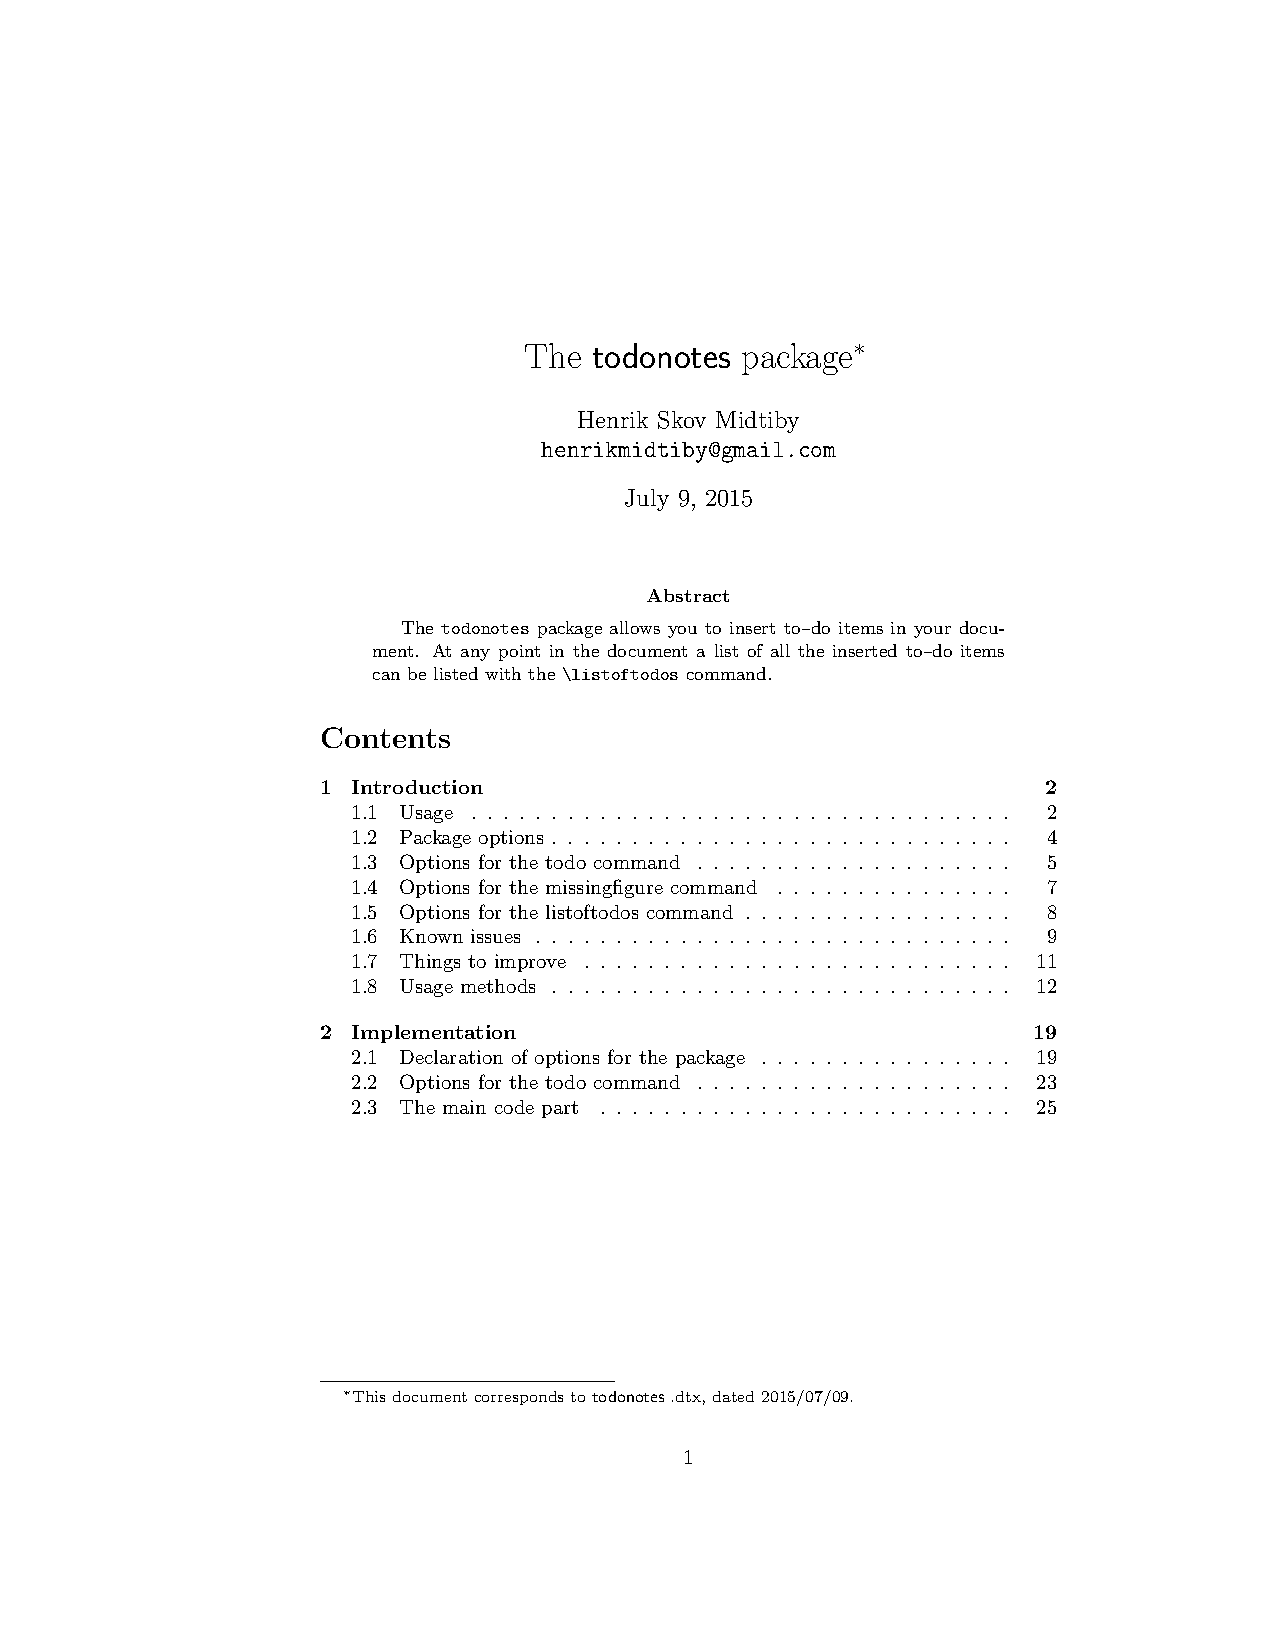
\includepdf[pages=1-3,scale=0.8,frame=true,pagecommand={}]{anexos/todonotes.pdf}

% ---
% Para incluir sem gerar a quebra de página inicial no anexo
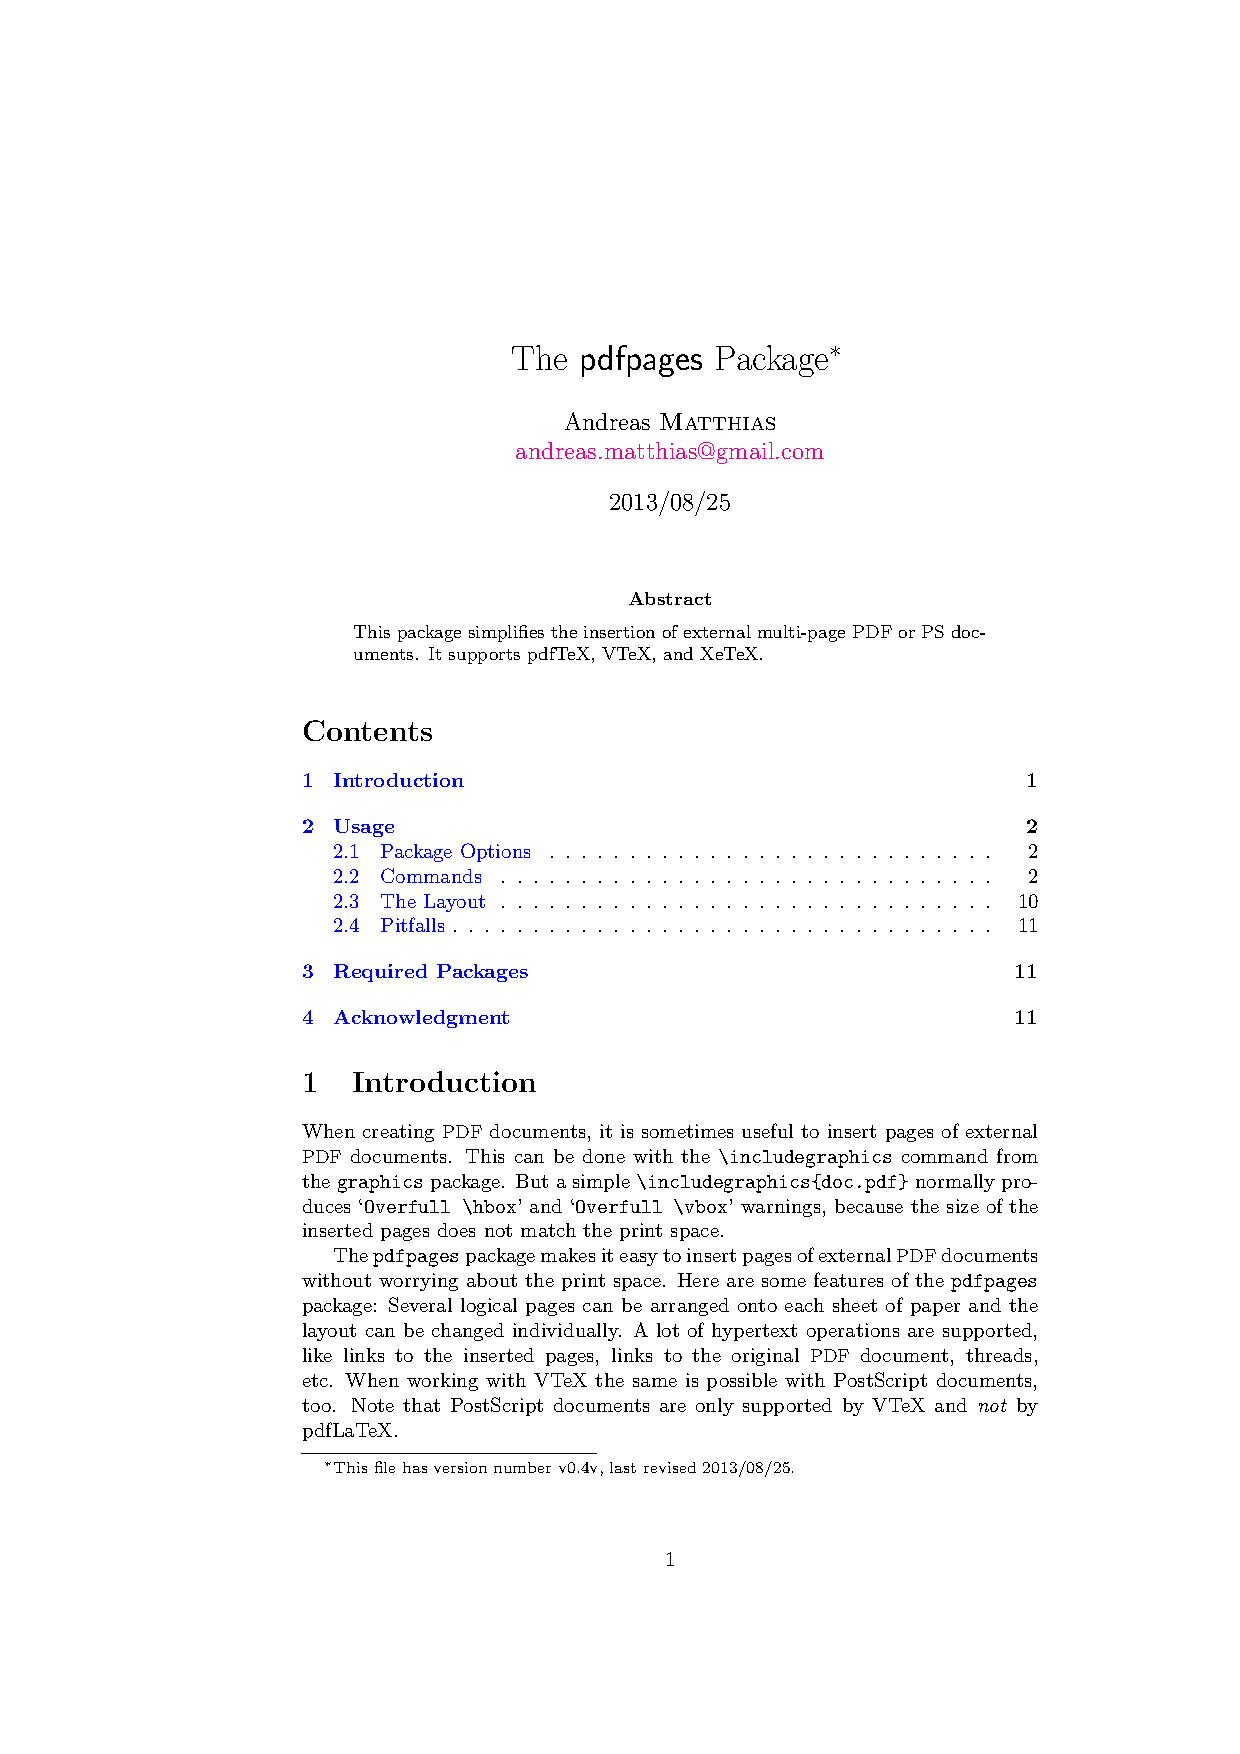
\includepdf[pages=1,scale=0.7,frame=true,pagecommand=\chapter{Manual pdfpages(parcial)}\label{manual-pdfpages}]{anexos/pdfpages.pdf}
\includepdf[pages=2-3,scale=0.8,frame=true,pagecommand={}]{anexos/pdfpages.pdf}

% ---
\chapter{Manual acronym(parcial)}
\index{pdf}
% somente algumas páginas para exemplo sem borda
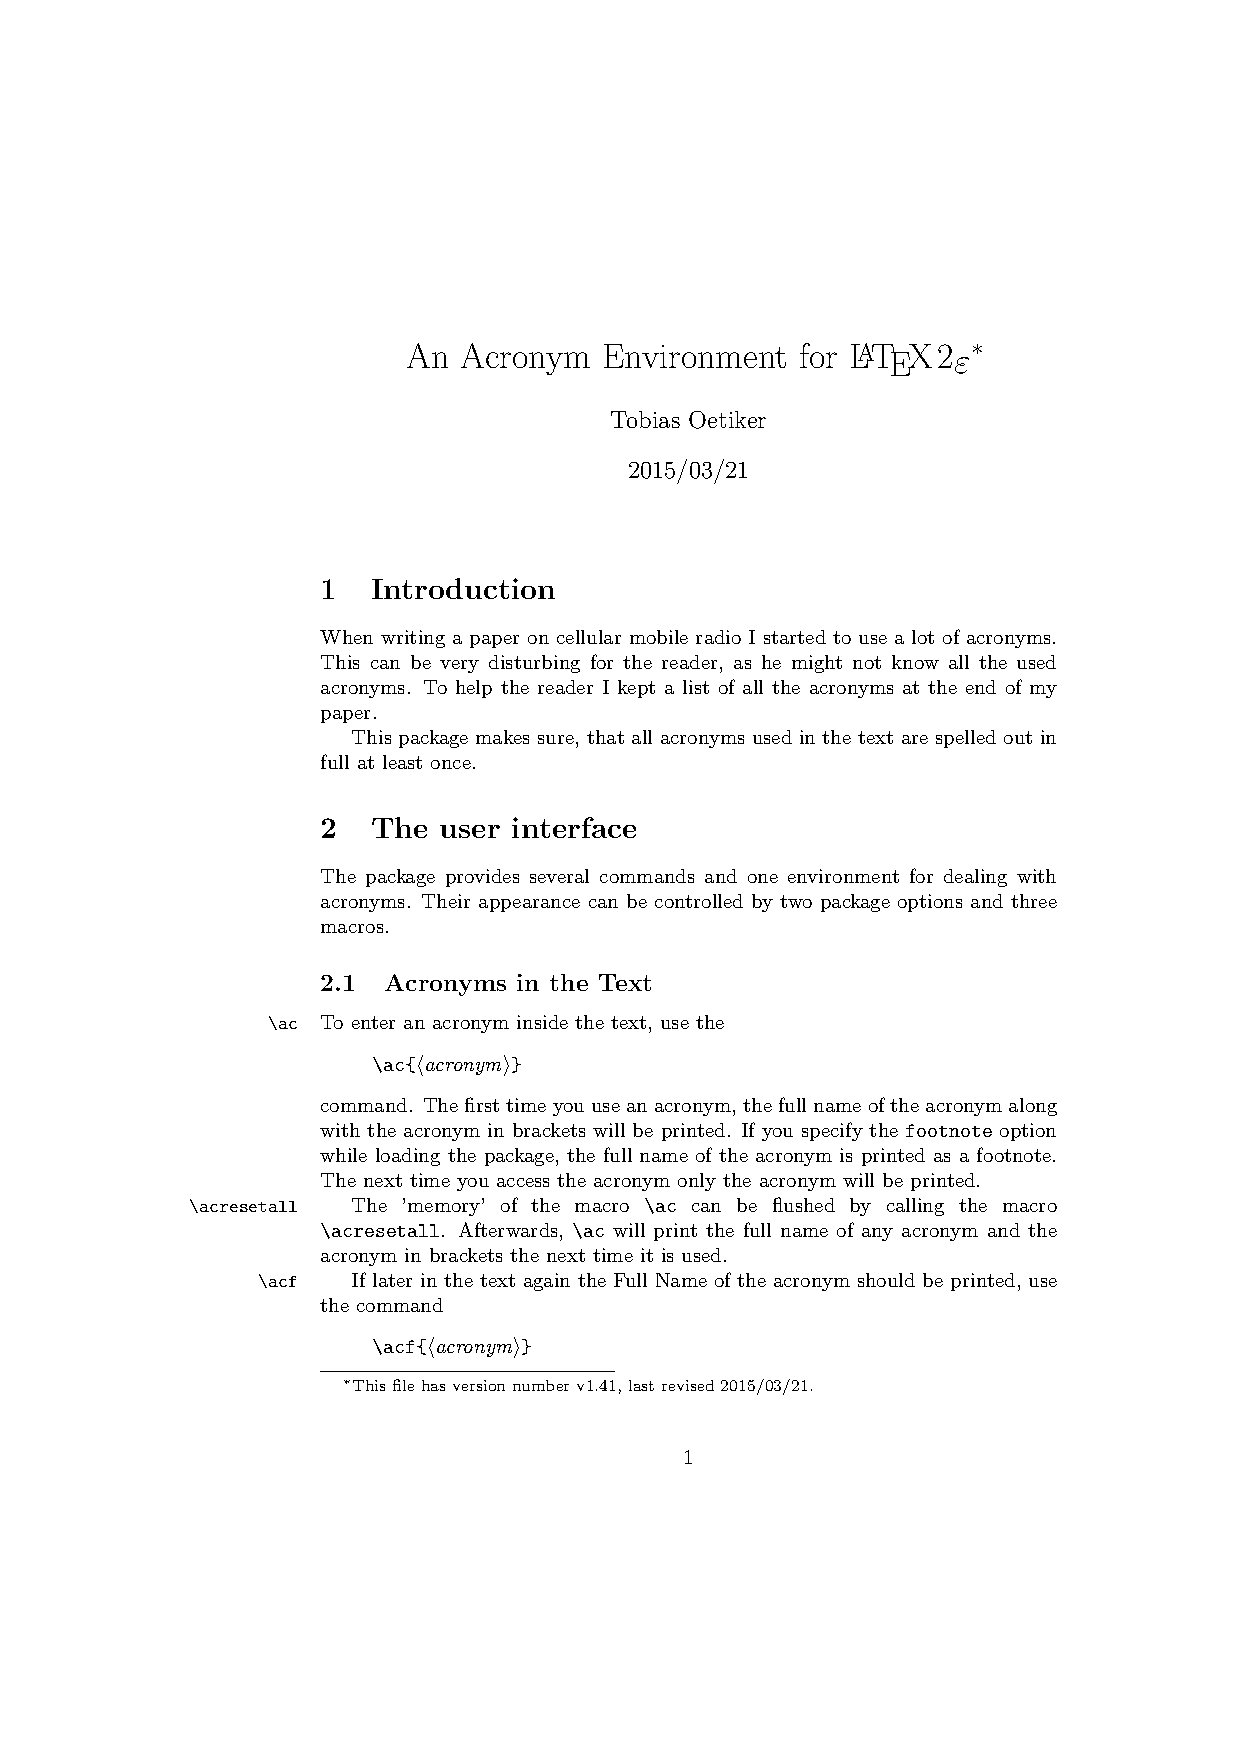
\includepdf[pages=1-3,frame=false,pagecommand={}]{anexos/acronym.pdf}



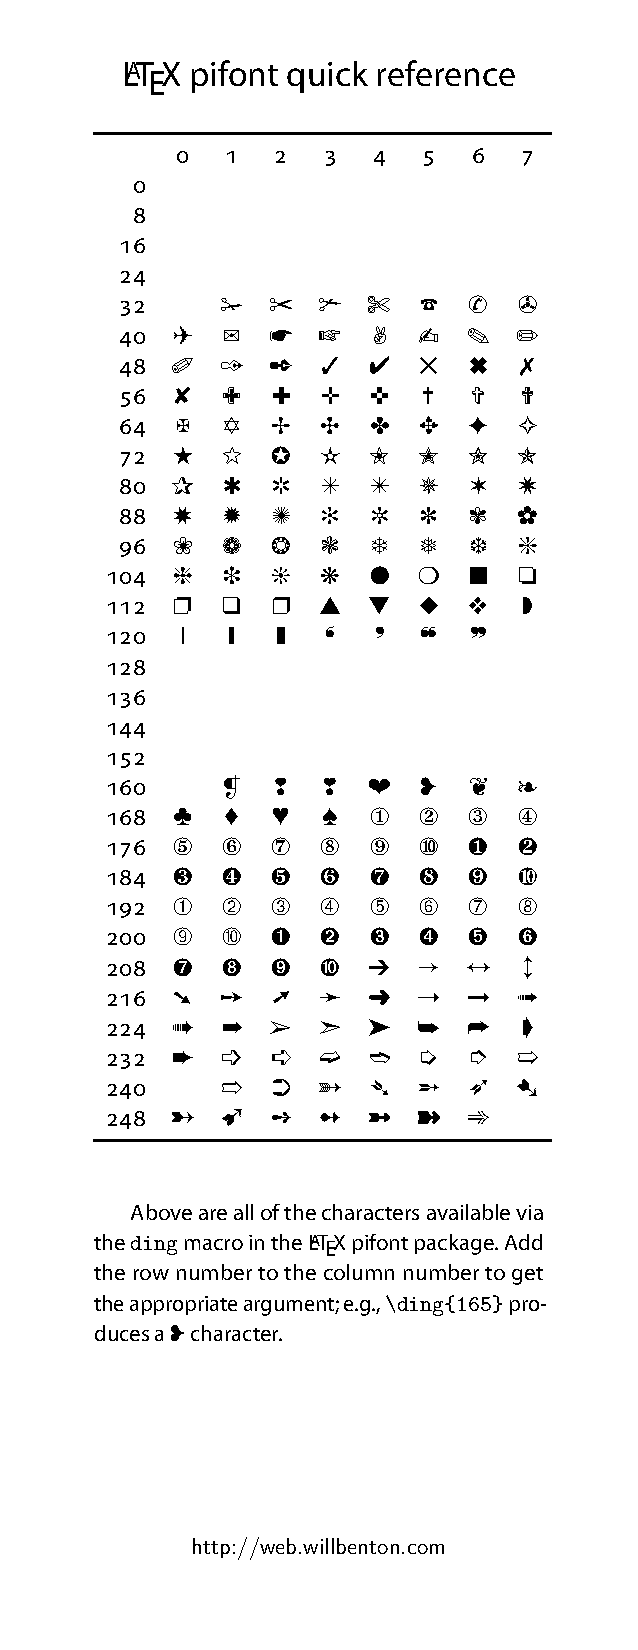
\includepdf[frame=true,scale=0.7,pagecommand=\chapter{Referência Rápida pifont}\label{pifont-quickref}]{anexos/pifont.pdf}


\end{anexosenv}



%---------------------------------------------------------------------
% INDICE REMISSIVO - Quando necessário 
% As palavras indexadas devem ser definidas com \index{} no texto
%---------------------------------------------------------------------
\phantompart
\printindex
\todonum[inline]{remover indice remissivo se não for necessário}

%---------------------------------------------------------------------

\end{document}